
\providecommand{\pandocbounded}[1]{#1}
\makeatletter
\def\maxwidth{\ifdim\Gin@nat@width>\linewidth\linewidth\else\Gin@nat@width\fi}
\def\maxheight{\ifdim\Gin@nat@height>\textheight\textheight\else\Gin@nat@height\fi}
\makeatother
\providecommand{\tightlist}{\setlength{\itemsep}{0pt}\setlength{\parskip}{0pt}}
\chapter{Lệnh thực thi có điều kiện}
\section{Chương 4 Lệnh thực thi có điều kiện (Conditional
Execution)}\label{chux1b0ux1a1ng-4-lux1ec7nh-thux1ef1c-thi-cuxf3-ux111iux1ec1u-kiux1ec7n-conditional-execution}

\subsection{Lệnh if/else}\label{lux1ec7nh-ifelse}

\begin{itemize}
\tightlist
\item
  Các toán tử quan hệ (Relational Operators)
\item
  Các lệnh if/else lồng nhau (Nested if/else Statements)
\item
  Sự bằng nhau của đối tượng (Object Equality)
\item
  Tối ưu hóa lệnh if/else (Factoring if/else Statements)
\item
  Kiểm tra nhiều điều kiện (Testing Multiple Conditions)
\end{itemize}

\subsection{Các thuật toán tích lũy (Cumulative
Algorithms)}\label{cuxe1c-thuux1eadt-touxe1n-tuxedch-lux169y-cumulative-algorithms}

\begin{itemize}
\tightlist
\item
  Tính tổng tích lũy (Cumulative Sum)
\item
  Vòng lặp tìm Min/Max
\item
  Tính tổng tích lũy với if
\item
  Sai số làm tròn (Roundoff Errors)
\end{itemize}

\subsection{Xử lý văn bản (Text
Processing)}\label{xux1eed-luxfd-vux103n-bux1ea3n-text-processing}

\begin{itemize}
\tightlist
\item
  Kiểu char
\end{itemize}

\begin{center}

\includegraphics[width=\maxwidth,height=\maxheight,width=0.9\linewidth]{Figures/img_p216_0.png}
\end{center}

\begin{itemize}
\tightlist
\item
  char so với int
\item
  Các thuật toán xử lý văn bản tích lũy
\item
  System.out.printf
\end{itemize}

\subsection{Các phương thức có lệnh thực thi có điều
kiện}\label{cuxe1c-phux1b0ux1a1ng-thux1ee9c-cuxf3-lux1ec7nh-thux1ef1c-thi-cuxf3-ux111iux1ec1u-kiux1ec7n}

\begin{itemize}
\tightlist
\item
  Tiền điều kiện và hậu điều kiện (Preconditions and Postconditions)
\item
  Ném ngoại lệ (Throwing Exceptions)
\item
  Xem lại giá trị trả về
\item
  Lập luận về các đường dẫn (Reasoning about Paths)
\end{itemize}

\subsection{Nghiên cứu điển hình: Chỉ số khối cơ thể (Body Mass
Index)}\label{nghiuxean-cux1ee9u-ux111iux1ec3n-huxecnh-chux1ec9-sux1ed1-khux1ed1i-cux1a1-thux1ec3-body-mass-index}

\begin{itemize}
\tightlist
\item
  Giải pháp không có cấu trúc cho một người
\item
  Giải pháp không có cấu trúc cho hai người
\item
  Giải pháp có cấu trúc cho hai người
\item
  Kinh nghiệm thiết kế thủ tục (Procedural Design Heuristics)
\end{itemize}

\subsection{Giới thiệu}\label{giux1edbi-thiux1ec7u}

Trong vài chương trước, bạn đã thấy cách giải quyết các bài toán lập
trình phức tạp bằng cách sử dụng các vòng lặp \texttt{for} để lặp lại
các tác vụ nhất định nhiều lần. Bạn cũng đã thấy cách đưa một số tính
linh hoạt vào các chương trình của mình bằng cách sử dụng các hằng số
lớp (class constants) và cách đọc các giá trị được người dùng nhập bằng
đối tượng \texttt{Scanner}.

\begin{center}

\includegraphics[width=\maxwidth,height=\maxheight,width=0.9\linewidth]{Figures/img_p217_0.png}
\end{center}

Bây giờ, chúng ta sẽ khám phá một kỹ thuật mạnh mẽ hơn nhiều để viết mã
có thể thích ứng với các tình huống khác nhau.

Trong chương này, chúng ta sẽ xem xét việc thực thi có điều kiện
(conditional execution) dưới dạng một cấu trúc điều khiển được gọi là
lệnh \texttt{if/else}. Với các lệnh \texttt{if/else}, bạn có thể hướng
dẫn máy tính thực thi các dòng mã khác nhau tùy thuộc vào việc các điều
kiện nhất định có đúng hay không. Lệnh \texttt{if/else}, giống như vòng
lặp \texttt{for}, mạnh mẽ đến mức bạn sẽ tự hỏi làm thế nào mà bạn xoay
sở viết được các chương trình mà không có nó.

Chương này cũng sẽ mở rộng hiểu biết của bạn về các tình huống lập trình
phổ biến. Nó bao gồm việc khám phá các kỹ thuật vòng lặp mà chúng ta
chưa xem xét và bao gồm cuộc thảo luận về các vấn đề xử lý văn bản. Việc
thêm thực thi có điều kiện vào vốn kiến thức của bạn cũng sẽ yêu cầu
chúng ta xem xét lại các phương thức, tham số và giá trị trả về để bạn
có thể hiểu rõ hơn về một số điểm tinh tế. Chương này kết thúc với một
số quy tắc ngón tay cái (rules of thumb) giúp chúng ta thiết kế các
chương trình thủ tục tốt hơn.

\subsection{Lệnh if/else}\label{lux1ec7nh-ifelse-1}

Bạn sẽ thường thấy mình viết đoạn mã mà bạn muốn thực thi một số lần
nhưng không phải là mọi lúc. Ví dụ, nếu bạn đang viết một chương trình
chơi game, bạn có thể muốn in một thông báo mỗi khi người dùng đạt điểm
cao mới và lưu trữ điểm đó. Bạn có thể hoàn thành việc này bằng cách đặt
hai dòng mã cần thiết bên trong một lệnh \texttt{if}:

\begin{verbatim}
if (currentScore > maxScore) {
    System.out.println("A new high score!");
    maxScore = currentScore;
}
\end{verbatim}

Ý tưởng là đôi khi bạn sẽ muốn thực thi hai dòng mã bên trong lệnh
\texttt{if}, nhưng không phải lúc nào cũng vậy. Biểu thức kiểm tra
(test) trong ngoặc đơn xác định xem các câu lệnh bên trong lệnh
\texttt{if} có được thực thi hay không. Nói cách khác, biểu thức kiểm
tra mô tả các điều kiện mà chúng ta muốn thực thi đoạn mã.

Dạng chung của lệnh \texttt{if} như sau:

\begin{verbatim}
if (<biểu thức kiểm tra>) {
    <câu lệnh>;
    <câu lệnh>;
    ...
    <câu lệnh>;
}
\end{verbatim}

Lệnh \texttt{if}, giống như vòng lặp \texttt{for}, là một cấu trúc điều
khiển. Lưu ý rằng một lần nữa chúng ta lại thấy một từ khóa Java
(\texttt{if}) theo sau là dấu ngoặc đơn và một cặp dấu ngoặc nhọn bao
quanh một chuỗi các câu lệnh được điều khiển.

Sơ đồ trong Hình 4.1 chỉ ra luồng điều khiển của lệnh \texttt{if} đơn
giản. Máy tính thực hiện biểu thức kiểm tra và nếu nó đánh giá là
\texttt{true} (đúng), máy tính sẽ thực thi các câu lệnh được điều khiển.
Nếu biểu thức kiểm tra đánh giá là \texttt{false} (sai), máy tính sẽ bỏ
qua các câu lệnh được điều khiển.

Hình 4.1 Luồng của lệnh \texttt{if}

\begin{center}

\includegraphics[width=\maxwidth,height=\maxheight,width=0.9\linewidth]{Figures/img_p221_0.png}
\end{center}

Bạn sẽ sử dụng lệnh \texttt{if} đơn giản khi bạn có mã mà bạn muốn thực
thi đôi khi và bỏ qua vào những lúc khác. Java cũng có một biến thể được
gọi là lệnh \texttt{if/else} cho phép bạn chọn giữa hai phương án thay
thế. Giả sử, ví dụ, bạn muốn gán biến tên là \texttt{answer} bằng căn
bậc hai của một số:

\begin{verbatim}
answer = Math.sqrt(number);
\end{verbatim}

Bạn không muốn yêu cầu căn bậc hai nếu số đó là số âm. Để tránh sự cố
tiềm ẩn này, bạn có thể sử dụng một lệnh \texttt{if} đơn giản:

\begin{center}
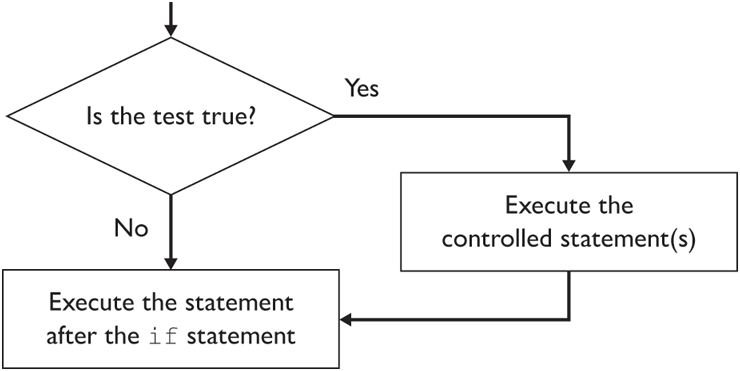
\includegraphics[width=\maxwidth,height=\maxheight,width=0.9\linewidth]{Figures/img_p222_0.png}
\end{center}

\begin{verbatim}
if (number >= 0) {
    answer = Math.sqrt(number);
}
\end{verbatim}

Đoạn mã này sẽ tránh việc yêu cầu căn bậc hai của một số âm, nhưng nó sẽ
gán giá trị gì cho \texttt{answer} nếu \texttt{number} là số âm? Trong
trường hợp này, có lẽ bạn sẽ muốn gán một giá trị cho \texttt{answer}
theo cách này hay cách khác. Giả sử bạn muốn \texttt{answer} là
\texttt{-1} khi \texttt{number} là số âm. Bạn có thể diễn đạt cặp phương
án thay thế này bằng lệnh \texttt{if/else} sau:

\begin{verbatim}
if (number >= 0) {
    answer = Math.sqrt(number);
} else {
    answer = -1;
}
\end{verbatim}

Lệnh \texttt{if/else} cung cấp hai phương án thay thế và thực thi một
hoặc phương án kia. Vì vậy, trong đoạn mã trên, bạn biết rằng
\texttt{answer} sẽ được gán một giá trị bất kể \texttt{number} dương hay
âm.

Dạng chung của lệnh \texttt{if/else} là:

\begin{verbatim}
if (<biểu thức kiểm tra>) {
    <câu lệnh>;
    <câu lệnh>;
    ...
    <câu lệnh>;
} else {
    <câu lệnh>;
    <câu lệnh>;
    ...
    <câu lệnh>;
}
\end{verbatim}

Cấu trúc điều khiển này khác thường ở chỗ nó có hai tập hợp các câu lệnh
được điều khiển và hai từ khóa khác nhau (\texttt{if} và \texttt{else}).
Hình 4.2 chỉ ra luồng điều khiển. Máy tính thực hiện biểu thức kiểm tra
và tùy thuộc vào việc mã đánh giá là \texttt{true} hay \texttt{false},
nó sẽ thực thi một trong hai nhóm câu lệnh.

Hình 4.2 Luồng của lệnh \texttt{if/else}

\begin{center}

\includegraphics[width=\maxwidth,height=\maxheight,width=0.9\linewidth]{Figures/img_p224_0.png}
\end{center}

Cũng giống như trường hợp của vòng lặp \texttt{for}, nếu bạn có một câu
lệnh duy nhất để thực thi, bạn không cần phải bao gồm dấu ngoặc nhọn.
Tuy nhiên, quy ước của Java là bao gồm các dấu ngoặc nhọn ngay cả khi
bạn không cần chúng, và chúng tôi tuân theo quy ước đó trong cuốn sách
này.

\subsubsection{Các toán tử quan hệ (Relational
Operators)}\label{cuxe1c-touxe1n-tux1eed-quan-hux1ec7-relational-operators}

Một lệnh \texttt{if/else} được điều khiển bởi một biểu thức kiểm tra
(test). Các biểu thức kiểm tra đơn giản so sánh hai biểu thức để xem
liệu chúng có liên quan theo một cách nào đó không. Bản thân các biểu
thức kiểm tra như vậy là các biểu thức có dạng sau đây và đánh giá thành
\texttt{true} hoặc \texttt{false}:

\texttt{\textless{}biểu\ thức\textgreater{}\ \textless{}toán\ tử\ quan\ hệ\textgreater{}\ \textless{}biểu\ thức\textgreater{}}

\begin{center}
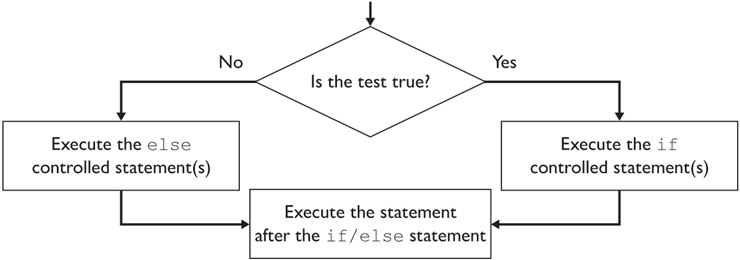
\includegraphics[width=\maxwidth,height=\maxheight,width=0.9\linewidth]{Figures/img_p225_0.png}
\end{center}

Để đánh giá một biểu thức kiểm tra có dạng này, trước tiên hãy đánh giá
hai biểu thức, sau đó xem liệu quan hệ đã cho có thỏa mãn (holds) giữa
giá trị bên trái và giá trị bên phải hay không. Nếu quan hệ thỏa mãn,
biểu thức kiểm tra đánh giá thành \texttt{true}. Nếu không, biểu thức
kiểm tra đánh giá thành \texttt{false}.

Các toán tử quan hệ được liệt kê trong Bảng 4.1. Lưu ý rằng toán tử bằng
(equality operator) bao gồm hai dấu bằng (\texttt{==}), để phân biệt nó
với toán tử gán (assignment operator) (\texttt{=}).

Bảng 4.1 Các toán tử quan hệ

\begin{center}

\includegraphics[width=\maxwidth,height=\maxheight,width=0.9\linewidth]{Figures/img_p226_0.png}
\end{center}

Bởi vì chúng ta sử dụng các toán tử quan hệ như một cách mới để tạo
thành các biểu thức, chúng ta phải xem xét lại độ ưu tiên (precedence).
Bảng 4.2 là phiên bản cập nhật của Bảng 2.5 bao gồm các toán tử mới này.
Bạn sẽ thấy rằng, về mặt kỹ thuật, các phép so sánh bằng có mức độ ưu
tiên hơi khác so với các toán tử quan hệ khác, nhưng cả hai nhóm toán tử
đều có độ ưu tiên thấp hơn các toán tử số học.

Bảng 4.2 Độ ưu tiên của các toán tử trong Java

Hãy xem xét một ví dụ. Biểu thức sau đây được tạo thành từ các hằng số
\texttt{3}, \texttt{2}, và \texttt{9} và chứa các phép tính cộng, nhân,
và phép toán bằng:

\begin{verbatim}
3 + 2 * 2 == 9
\end{verbatim}

\begin{center}
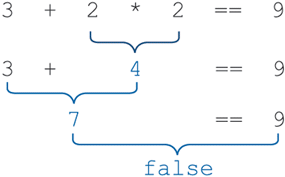
\includegraphics[width=\maxwidth,height=\maxheight,width=0.9\linewidth]{Figures/img_p227_0.png}
\end{center}

Phép toán nào được thực hiện trước? Vì các toán tử quan hệ có mức độ ưu
tiên thấp hơn các toán tử số học, phép nhân được thực hiện trước, sau đó
là phép cộng, sau đó là biểu thức kiểm tra bằng. Nói cách khác, Java sẽ
thực hiện tất cả các phép toán ``toán học'' trước khi nó kiểm tra bất kỳ
mối quan hệ nào. Lược đồ độ ưu tiên này giải phóng bạn khỏi việc phải
đặt dấu ngoặc đơn quanh các vế trái và vế phải của một biểu thức kiểm
tra sử dụng toán tử quan hệ. Khi bạn tuân theo các quy tắc độ ưu tiên
của Java, biểu thức mẫu được đánh giá như sau:

Bạn có thể đặt các biểu thức tùy ý ở hai bên của toán tử quan hệ, miễn
là các kiểu dữ liệu tương thích. Dưới đây là một biểu thức kiểm tra với
các biểu thức phức tạp ở cả hai bên:

\begin{verbatim}
(2 - 3 * 8) / (435 % (7 * 2)) <= 3.8 - 4.5 / (2.2 * 3.8)
\end{verbatim}

Bạn có thể kiểm tra các toán tử quan hệ trong JShell, như được hiển thị
trong tương tác sau:

\begin{verbatim}
jshell> int a = 3; 
a ==> 3
jshell> int b = 2;
b ==> 2
jshell> a > b
$3 ==> true
jshell> a > b * b
$4 ==> false
jshell> a - 1 == b
$5 ==> true
\end{verbatim}

Một hạn chế của các toán tử quan hệ là chúng chỉ nên được sử dụng với dữ
liệu nguyên thủy (primitive data). Ở phần sau của chương này, chúng ta
sẽ nói về cách so sánh sự bằng nhau của các đối tượng (objects) và trong
chương sau, chúng ta sẽ thảo luận về cách thực hiện các phép so sánh nhỏ
hơn và lớn hơn đối với các đối tượng.

\subsubsection{Các lệnh if/else lồng nhau (Nested if/else
Statements)}\label{cuxe1c-lux1ec7nh-ifelse-lux1ed3ng-nhau-nested-ifelse-statements}

\begin{center}

\includegraphics[width=\maxwidth,height=\maxheight,width=0.9\linewidth]{Figures/img_p229_0.png}
\end{center}

Nhiều người mới bắt đầu thường viết mã trông như thế này:

\begin{verbatim}
if (<biểu thức kiểm tra 1>) {
    <câu lệnh 1>;
}
if (<biểu thức kiểm tra 2>) {
    <câu lệnh 2>;
}
if (<biểu thức kiểm tra 3>) {
    <câu lệnh 3>;
}
\end{verbatim}

Cấu trúc tuần tự này phù hợp nếu bạn muốn thực thi bất kỳ tổ hợp nào của
ba câu lệnh. Ví dụ, bạn có thể viết đoạn mã này trong một chương trình
cho một bảng câu hỏi với ba phần tùy chọn, bất kỳ tổ hợp nào trong số đó
cũng có thể áp dụng cho một người cụ thể. Hình 4.3 cho thấy luồng của mã
\texttt{if} tuần tự. Lưu ý rằng máy tính có thể không thực thi câu lệnh
được điều khiển nào (nếu tất cả các biểu thức kiểm tra đều là
\texttt{false}), chỉ thực thi một câu lệnh (nếu tình cờ chỉ có một biểu
thức kiểm tra là \texttt{true}), hoặc thực thi nhiều hơn một câu lệnh
(nếu nhiều biểu thức kiểm tra là \texttt{true}).

Hình 4.3 Luồng của các lệnh \texttt{if} tuần tự (sequential ifs)

\begin{center}

\includegraphics[width=\maxwidth,height=\maxheight,width=0.9\linewidth]{Figures/img_p229_1.png}
\end{center}

\begin{center}
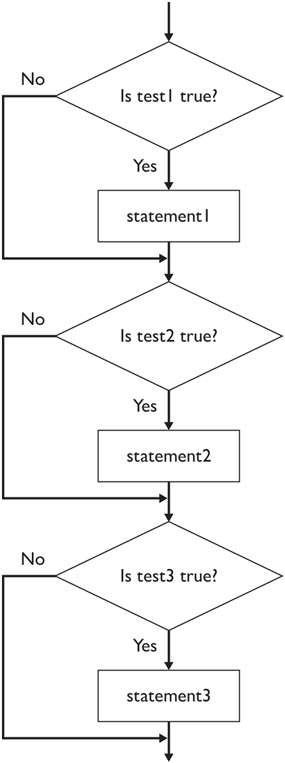
\includegraphics[width=\maxwidth,height=\maxheight,width=0.9\linewidth]{Figures/img_p231_0.png}
\end{center}

Tuy nhiên, thông thường bạn chỉ muốn thực thi một trong một chuỗi các
câu lệnh. Trong những trường hợp như vậy, tốt hơn là lồng các lệnh
\texttt{if}, xếp chúng cái này bên trong cái kia:

\begin{verbatim}
if (<biểu thức kiểm tra 1>) {
    <câu lệnh 1>;
} else {
    if (<biểu thức kiểm tra 2>) {
        <câu lệnh 2>;
    } else {
        if (<biểu thức kiểm tra 3>) {
            <câu lệnh 3>;
        }
    }
}
\end{verbatim}

Khi bạn sử dụng cấu trúc này, bạn có thể chắc chắn rằng máy tính sẽ thực
thi nhiều nhất một câu lệnh: câu lệnh tương ứng với biểu thức kiểm tra
đầu tiên đánh giá thành \texttt{true}. Nếu không có biểu thức kiểm tra
nào đánh giá thành \texttt{true}, không có câu lệnh nào được thực thi.
Nếu mục tiêu của bạn là thực thi nhiều nhất một câu lệnh, cấu trúc này
thích hợp hơn so với các lệnh \texttt{if} tuần tự. Nó làm giảm khả năng
xảy ra lỗi và đơn giản hóa quá trình kiểm thử.

Như bạn có thể thấy, việc lồng các lệnh \texttt{if} như thế này dẫn đến
rất nhiều thụt lề (indentation). Việc thụt lề này không hữu ích lắm, vì
cấu trúc này thực sự nhằm mục đích cho phép chọn một trong nhiều phương
án thay thế. Phong cách K\&R cũng có một giải pháp cho việc này. Nếu một
\texttt{else} được theo sau bởi một \texttt{if}, chúng ta đặt chúng trên
cùng một dòng:

\begin{verbatim}
if (<biểu thức kiểm tra 1>) {
    <câu lệnh 1>;
} else if (<biểu thức kiểm tra 2>) {
    <câu lệnh 2>;
} else if (<biểu thức kiểm tra 3>) {
    <câu lệnh 3>;
}
\end{verbatim}

Khi bạn tuân theo quy ước này, tất cả các câu lệnh khác nhau đều xuất
hiện ở cùng một mức thụt lề. Chúng tôi khuyên bạn nên thụt lề các lệnh
\texttt{if/else} lồng nhau theo cách này.

Hình 4.4 cho thấy luồng của mã \texttt{if/else} lồng nhau. Lưu ý rằng
máy tính có thể thực thi một trong các câu lệnh được điều khiển (câu
lệnh đầu tiên đánh giá thành \texttt{true}) hoặc không thực thi câu lệnh
nào (nếu không có biểu thức kiểm tra nào đánh giá thành \texttt{true}).

Hình 4.4 Luồng của các lệnh \texttt{if} lồng nhau kết thúc bằng biểu
thức kiểm tra (ending in test)

\begin{center}

\includegraphics[width=\maxwidth,height=\maxheight,width=0.9\linewidth]{Figures/img_p233_0.png}
\end{center}

Trong một biến thể của cấu trúc này, câu lệnh cuối cùng được điều khiển
bởi một \texttt{else} thay vì một biểu thức kiểm tra:

\begin{verbatim}
if (<biểu thức kiểm tra 1>) {
    <câu lệnh 1>;
} else if (<biểu thức kiểm tra 2>) {
    <câu lệnh 2>;
\end{verbatim}

\begin{center}
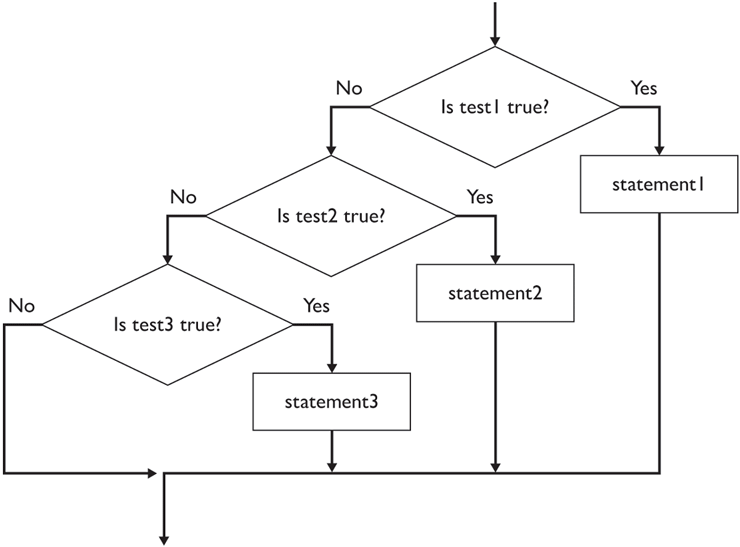
\includegraphics[width=\maxwidth,height=\maxheight,width=0.9\linewidth]{Figures/img_p234_0.png}
\end{center}

\begin{verbatim}
} else {
    <câu lệnh 3>;
}
\end{verbatim}

Trong cấu trúc này, máy tính sẽ luôn chọn nhánh cuối cùng khi tất cả các
biểu thức kiểm tra đều sai, và do đó cấu trúc sẽ luôn thực thi chính xác
một trong ba câu lệnh. Hình 4.5 cho thấy luồng của mã \texttt{if/else}
lồng nhau đã được sửa đổi này.

Hình 4.5 Luồng của các lệnh \texttt{if} lồng nhau kết thúc bằng
\texttt{else}

\begin{center}

\includegraphics[width=\maxwidth,height=\maxheight,width=0.9\linewidth]{Figures/img_p235_0.png}
\end{center}

\begin{center}
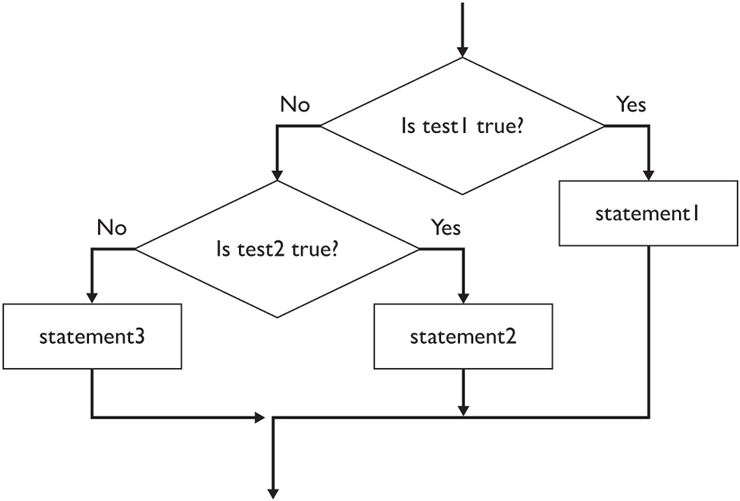
\includegraphics[width=\maxwidth,height=\maxheight,width=0.9\linewidth]{Figures/img_p235_1.png}
\end{center}

Để khám phá những biến thể này, hãy xem xét tác vụ yêu cầu máy tính cho
biết một số là dương, âm, hay bằng 0. Bạn có thể cấu trúc tác vụ này
thành ba lệnh \texttt{if} đơn giản như sau:

\begin{verbatim}
if (number > 0) {
    System.out.println("Number is positive.");
}
if (number == 0) {
    System.out.println("Number is zero.");
}
if (number < 0) {
    System.out.println("Number is negative.");
}
\end{verbatim}

Để xác định có bao nhiêu câu lệnh \texttt{println} có khả năng được thực
thi, bạn phải dừng lại và suy nghĩ về các biểu thức kiểm tra đang được
thực hiện. Nhưng bạn không nên phải tốn nhiều công sức như vậy để hiểu
mã này. Mã sẽ rõ ràng hơn nếu bạn lồng các lệnh \texttt{if}:

\begin{verbatim}
if (number > 0) {
    System.out.println("Number is positive.");
} else if (number == 0) {
    System.out.println("Number is zero.");
} else if (number < 0) {
    System.out.println("Number is negative.");
}
\end{verbatim}

Tuy nhiên, giải pháp này có một vấn đề. Bạn biết rằng bạn muốn thực thi
một và chỉ một câu lệnh \texttt{println}, nhưng cấu trúc lồng nhau này
không loại trừ khả năng không có câu lệnh nào được thực thi (điều này sẽ
xảy ra nếu cả ba biểu thức kiểm tra đều sai). Tất nhiên, với các biểu
thức kiểm tra cụ thể này thì điều đó sẽ không bao giờ xảy ra: Nếu một số
không phải là dương cũng không phải là 0, thì nó phải là âm. Do đó, biểu
thức kiểm tra cuối cùng ở đây là không cần thiết và gây hiểu lầm. Bạn
phải suy nghĩ về các biểu thức kiểm tra để xác định liệu có thể tất cả
ba biểu thức kiểm tra đều sai và cả ba nhánh đều bị bỏ qua hay không.

Trong trường hợp này, giải pháp tốt nhất là phương pháp tiếp cận
\texttt{if/else} lồng nhau với một nhánh cuối cùng luôn được chọn nếu
hai biểu thức kiểm tra đầu tiên đều sai:

\begin{verbatim}
if (number > 0) {
    System.out.println("Number is positive.");
} else if (number == 0) {
    System.out.println("Number is zero.");
} else {
    System.out.println("Number is negative.");
}
\end{verbatim}

Bạn có thể nhìn lướt qua cấu trúc này và thấy ngay rằng chính xác một
câu lệnh \texttt{println} sẽ được thực thi. Bạn không cần phải nhìn vào
các biểu thức kiểm tra đang được thực hiện để nhận ra điều này; đó là
thuộc tính của loại cấu trúc \texttt{if/else} lồng nhau này. Nếu muốn,
bạn có thể bao gồm một chú thích để làm rõ điều gì đang diễn ra:

\begin{verbatim}
if (number > 0) {
    System.out.println("Number is positive.");
} else if (number == 0) {
    System.out.println("Number is zero.");
} else { // number must be negative 
    System.out.println("Number is negative.");
}
\end{verbatim}

Một lợi ích cuối cùng của phương pháp này là tính hiệu quả (efficiency).
Khi mã bao gồm ba lệnh \texttt{if} đơn giản, máy tính sẽ luôn thực hiện
cả ba bài kiểm tra. Khi mã sử dụng phương pháp \texttt{if/else} lồng
nhau, máy tính chỉ thực hiện các biểu thức kiểm tra cho đến khi tìm thấy
sự trùng khớp, điều này là việc sử dụng tài nguyên tốt hơn. Ví dụ, trong
đoạn mã trước, chúng ta chỉ cần thực hiện một bài kiểm tra cho các số
dương và nhiều nhất là hai bài kiểm tra tổng thể.

Khi bạn thấy mình đang viết mã để chọn giữa các phương án thay thế như
thế này, bạn phải phân tích bài toán cụ thể để tìm ra bạn muốn thực thi
có khả năng bao nhiêu nhánh. Nếu việc kết hợp các nhánh nào được chọn
không quan trọng, hãy sử dụng các lệnh \texttt{if} tuần tự. Nếu bạn muốn
chọn một hoặc không chọn nhánh nào, hãy sử dụng các lệnh
\texttt{if/else} lồng nhau với một biểu thức kiểm tra cho mỗi câu lệnh.
Nếu bạn muốn chọn chính xác một nhánh, hãy sử dụng các lệnh
\texttt{if/else} lồng nhau với một nhánh cuối cùng được điều khiển bởi
một \texttt{else} thay vì một biểu thức kiểm tra. Bảng 4.3 tóm tắt những
lựa chọn này.

Bảng 4.3 Các tùy chọn if/else

\begin{center}

\includegraphics[width=\maxwidth,height=\maxheight,width=0.9\linewidth]{Figures/img_p239_0.png}
\end{center}

\subsubsection{LỖI LẬP TRÌNH PHỔ
BIẾN}\label{lux1ed7i-lux1eadp-truxecnh-phux1ed5-biux1ebfn}

\paragraph{Chọn sai cấu trúc
if/else}\label{chux1ecdn-sai-cux1ea5u-truxfac-ifelse}

Giả sử giáo viên của bạn nói rằng điểm số sẽ được xác định như sau: A
cho điểm \textgreater= 90 B cho điểm \textgreater= 80 C cho điểm
\textgreater= 70 D cho điểm \textgreater= 60 F cho điểm \textless{} 60

Bạn có thể chuyển đổi thang điểm này thành mã như sau:

\begin{verbatim}
String grade;
if (score >= 90) {
    grade = "A";
}
if (score >= 80) {
    grade = "B";
}
if (score >= 70) {
    grade = "C";
}
if (score >= 60) {
    grade = "D";
}
if (score < 60) {
    grade = "F";
}
\end{verbatim}

Tuy nhiên, nếu sau đó bạn cố gắng sử dụng biến \texttt{grade} sau đoạn
mã này, bạn sẽ nhận được lỗi này từ trình biên dịch:
\texttt{variable\ grade\ might\ not\ have\ been\ initialized} Đây là một
manh mối cho thấy có một vấn đề. Trình biên dịch Java đang nói rằng nó
tin rằng có những đường dẫn qua mã này sẽ khiến biến \texttt{grade}
không được khởi tạo. Thực tế, biến sẽ luôn được khởi tạo, nhưng trình
biên dịch không thể tìm ra điều này. Chúng ta có thể sửa vấn đề này bằng
cách cung cấp một giá trị ban đầu cho \texttt{grade}:

\begin{verbatim}
String grade = "no grade";
\end{verbatim}

Sự thay đổi này cho phép mã biên dịch được. Nhưng nếu bạn biên dịch và
chạy chương trình, bạn sẽ thấy rằng nó chỉ đưa ra hai mức điểm: D và F.
Bất kỳ ai có điểm số từ 60 trở lên đều nhận được điểm D và bất kỳ ai có
điểm số dưới 60 đều nhận được điểm F. Và mặc dù trình biên dịch phàn nàn
rằng có một đường dẫn có thể khiến \texttt{grade} không được khởi tạo,
nhưng không ai bao giờ nhận được mức điểm là ``no grade''.

Vấn đề ở đây là bạn muốn thực thi chính xác một trong các câu lệnh gán,
nhưng khi bạn sử dụng các lệnh \texttt{if} tuần tự, chương trình có thể
thực thi lần lượt một vài lệnh trong số chúng. Ví dụ, nếu một sinh viên
có điểm số là 95, điểm của sinh viên đó được đặt thành \texttt{"A"}, sau
đó đặt lại thành \texttt{"B"}, sau đó đặt lại thành \texttt{"C"}, và
cuối cùng đặt lại thành \texttt{"D"}. Bạn có thể sửa vấn đề này bằng
cách sử dụng cấu trúc \texttt{if/else} lồng nhau:

\begin{verbatim}
String grade;
if (score >= 90) {
    grade = "A";
} else if (score >= 80) {
     grade = "B";
} else if (score >= 70) {
    grade = "C";
} else if (score >= 60) {
    grade = "D";
} else { // score < 60
    grade = "F";
}
\end{verbatim}

Bây giờ bạn không cần phải đặt \texttt{grade} thành \texttt{"no\ grade"}
vì trình biên dịch có thể thấy rằng bất kể đường dẫn nào được theo sau,
biến \texttt{grade} sẽ được gán một giá trị (chính xác một trong các
nhánh sẽ được thực thi).

\subsubsection{Sự bằng nhau của đối tượng (Object
Equality)}\label{sux1ef1-bux1eb1ng-nhau-cux1ee7a-ux111ux1ed1i-tux1b0ux1ee3ng-object-equality}

Ở phần trước trong chương này, bạn đã thấy rằng bạn có thể sử dụng các
toán tử \texttt{==} và \texttt{!=} để kiểm tra sự bằng nhau và không
bằng nhau tương ứng của dữ liệu nguyên thủy (primitive data). Thật không
may, các toán tử này không hoạt động theo cách bạn có thể mong đợi khi
bạn kiểm tra sự bằng nhau của các đối tượng như chuỗi (strings). Bạn sẽ
phải học một cách mới để kiểm tra sự bằng nhau của các đối tượng.

Ví dụ, bạn có thể viết mã như sau để đọc một token từ bảng điều khiển
(console) và gọi một trong hai phương thức khác nhau tùy thuộc vào việc
người dùng đã trả lời bằng ``yes'' hay ``no''. Nếu người dùng không nhập
từ nào, đoạn mã này được cho là sẽ in ra một thông báo lỗi:

\begin{verbatim}
System.out.print("yes or no? ");
String s = console.next();
if (s == "yes") {
    processYes();
} else if (s == "no") {
    processNo();
} else {
    System.out.println("You didn't type yes or no");
}
\end{verbatim}

Thật không may, đoạn mã này không hoạt động. Bất kể người dùng nhập gì,
chương trình này luôn in ra ``You didn't type yes or no''. Chúng ta sẽ
khám phá chi tiết trong Chương 8 lý do tại sao mã này không hoạt động.
Hiện tại, điều quan trọng cần biết là Java cung cấp một cách thứ hai để
kiểm tra sự bằng nhau dành cho việc sử dụng với các đối tượng. Mọi đối
tượng Java đều có một phương thức được gọi là \texttt{equals} nhận một
đối tượng khác làm đối số. Bạn có thể sử dụng phương thức này để hỏi một
đối tượng xem nó có bằng một đối tượng khác không. Ví dụ, chúng xuất
hiện trong sửa đoạn mã trước đó như sau:

\begin{center}

\includegraphics[width=\maxwidth,height=\maxheight,width=0.9\linewidth]{Figures/img_p243_0.png}
\end{center}

\begin{verbatim}
System.out.print("yes or no? ");
String s = console.next();
if (s.equals("yes")) {
    processYes();
} else if (s.equals("no")) {
    processNo();
} else {
    System.out.println("You didn't type yes or no");
}
\end{verbatim}

Hãy nhớ rằng khi bạn làm việc với chuỗi, bạn phải luôn gọi phương thức
\texttt{equals} thay vì sử dụng \texttt{==}.

Lớp \texttt{String} cũng có một biến thể đặc biệt của phương thức
\texttt{equals} có tên là \texttt{equalsIgnoreCase} để bỏ qua sự khác
biệt về chữ hoa chữ thường (uppercase so với lowercase). Ví dụ, bạn có
thể viết lại đoạn mã trước đó như sau để nhận dạng các phản hồi như
``Yes,'' ``YES,'' ``No,'' ``NO,'' ``yES'', và vân vân:

\begin{verbatim}
System.out.print("yes or no? ");
String s = console.next();
if (s.equalsIgnoreCase("yes")) {
    processYes();
} else if (s.equalsIgnoreCase("no")) {
    processNo();
} else {
    System.out.println("You didn't type yes or no");
}
\end{verbatim}

\subsubsection{Tối ưu hóa lệnh if/else (Factoring if/else
Statements)}\label{tux1ed1i-ux1b0u-huxf3a-lux1ec7nh-ifelse-factoring-ifelse-statements}

Giả sử bạn đang viết một chương trình chơi trò cá cược với người dùng và
bạn muốn đưa ra các cảnh báo khác nhau về số tiền mặt mà người dùng còn
lại. Cấu trúc \texttt{if/else} lồng nhau dưới đây phân biệt ba trường
hợp khác nhau: tiền ít hơn \$500, được coi là thấp; tiền từ \$500 đến
\$1000, được coi là ổn; và tiền trên \$1000, được coi là tốt. Lưu ý rằng
người dùng được đưa ra những lời khuyên khác nhau trong từng trường hợp:

\begin{center}

\includegraphics[width=\maxwidth,height=\maxheight,width=0.9\linewidth]{Figures/img_p245_0.png}
\end{center}

\begin{verbatim}
if (money < 500) {
    System.out.println("You have $" + money + " left.");
    System.out.print("Cash is dangerously low. Bet carefully.");
    System.out.print("How much do you want to bet? ");
    bet = console.nextInt();
} else if (money < 1000) {
    System.out.println("You have $" + money + " left.");
    System.out.print("Cash is somewhat low. Bet moderately.");
    System.out.print("How much do you want to bet? ");
    bet = console.nextInt();
} else {
\end{verbatim}

\begin{verbatim}
    System.out.println("You have $" + money + " left.");
    System.out.print("Cash is in good shape. Bet liberally.");
    System.out.print("How much do you want to bet? ");
    bet = console.nextInt();
}
\end{verbatim}

Cấu trúc này bị lặp lại và có thể được làm hiệu quả hơn bằng cách sử
dụng một kỹ thuật gọi là tối ưu hóa (factoring). Sử dụng kỹ thuật đơn
giản này, bạn rút các đoạn mã chung ra khỏi các nhánh khác nhau của cấu
trúc \texttt{if/else}. Trong đoạn mã trước, ba nhánh khác nhau có thể
thực thi, tùy thuộc vào giá trị của biến \texttt{money}. Bắt đầu bằng
cách viết ra chuỗi các hành động được thực hiện trong mỗi nhánh và so
sánh chúng, như trong Hình 4.6.

Hình 4.6 Các nhánh \texttt{if/else} trước khi tối ưu hóa

\begin{center}

\includegraphics[width=\maxwidth,height=\maxheight,width=0.9\linewidth]{Figures/img_p246_0.png}
\end{center}

\begin{center}
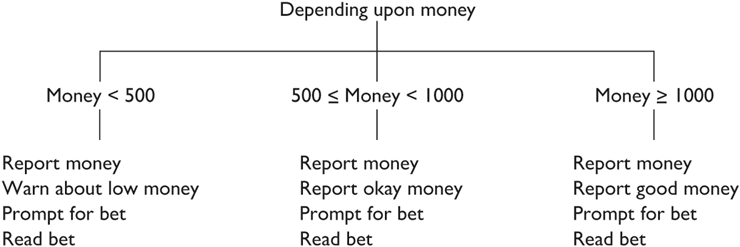
\includegraphics[width=\maxwidth,height=\maxheight,width=0.9\linewidth]{Figures/img_p246_1.png}
\end{center}

Bạn có thể tối ưu hóa ở cả đầu và cuối của một cấu trúc như thế này. Nếu
bạn nhận thấy câu lệnh đầu tiên trong mỗi nhánh là giống nhau, bạn rút
nó ra khỏi phần phân nhánh và đặt nó trước nhánh. Tương tự, nếu câu lệnh
cuối cùng trong mỗi nhánh là giống nhau, bạn rút nó ra khỏi phần phân
nhánh và đặt nó sau phần điều kiện. Bạn có thể rút câu lệnh đầu tiên
trong mỗi nhánh này và hai câu lệnh cuối cùng, như trong Hình 4.7.

Hình 4.7 Các nhánh \texttt{if/else} sau khi tối ưu hóa

\begin{center}

\includegraphics[width=\maxwidth,height=\maxheight,width=0.9\linewidth]{Figures/img_p247_0.png}
\end{center}

\begin{center}
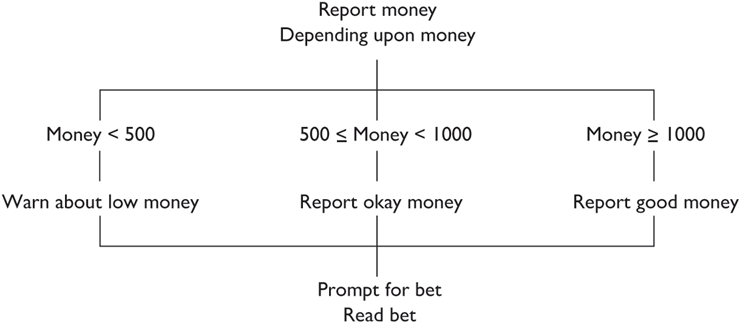
\includegraphics[width=\maxwidth,height=\maxheight,width=0.9\linewidth]{Figures/img_p247_1.png}
\end{center}

Do đó, đoạn mã trước có thể được rút gọn thành phiên bản súc tích hơn
sau:

\begin{verbatim}
System.out.println("You have $" + money + " left.");
if (money < 500) {
    System.out.print("Cash is dangerously low. Bet carefully.");
} else if (money < 1000) {
    System.out.print("Cash is somewhat low. Bet moderately.");
} else {
    System.out.print("Cash is in good shape. Bet liberally.");
}
System.out.print("How much do you want to bet? ");
bet = console.nextInt();
\end{verbatim}

\subsubsection{Kiểm tra nhiều điều kiện (Testing Multiple
Conditions)}\label{kiux1ec3m-tra-nhiux1ec1u-ux111iux1ec1u-kiux1ec7n-testing-multiple-conditions}

Khi bạn đang viết một chương trình, bạn thường thấy mình muốn kiểm tra
nhiều hơn một điều kiện. Ví dụ, giả sử bạn muốn chương trình thực hiện
một hành động cụ thể nếu một số nằm trong khoảng từ 1 đến 10. Bạn có thể
viết:

\begin{verbatim}
if (number >= 1) {
    if (number <= 10) {
        doSomething();
    }
}
\end{verbatim}

Trong những dòng mã này, bạn phải viết hai câu lệnh: một câu lệnh kiểm
tra xem số đó có lớn hơn hoặc bằng 1 hay không và một câu lệnh kiểm tra
xem số đó có nhỏ hơn hoặc bằng 10 hay không.

Java cung cấp một giải pháp thay thế hiệu quả: Bạn có thể kết hợp hai
bài kiểm tra bằng cách sử dụng một toán tử được gọi là toán tử logic AND
(logical AND operator), được viết bằng hai dấu và không có khoảng trắng
ở giữa (\texttt{\&\&}). Sử dụng toán tử AND, chúng ta có thể viết đoạn
mã trước đơn giản hơn:

\begin{verbatim}
if (number >= 1 && number <= 10) {
    doSomething();
}
\end{verbatim}

Đúng như tên gọi của nó, toán tử AND tạo thành một biểu thức kiểm tra
yêu cầu cả hai phần của biểu thức kiểm tra đều phải đánh giá thành
\texttt{true}. Có một toán tử tương tự được gọi là logic OR (logical OR)
đánh giá thành \texttt{true} nếu một trong hai biểu thức kiểm tra đánh
giá thành \texttt{true}. Toán tử logic OR được viết bằng cách sử dụng
hai ký tự gạch đứng (\texttt{\textbar{}\textbar{}}). Ví dụ, nếu bạn muốn
kiểm tra xem một biến \texttt{number} có bằng 1 hoặc 2 hay không, bạn có
thể viết:

\begin{verbatim}
if (number == 1 || number == 2) {
    processNumber(number);
}
\end{verbatim}

Chúng ta sẽ khám phá các toán tử logic AND và logic OR chi tiết hơn
trong chương tiếp theo.

\subsection{Các thuật toán tích lũy (Cumulative
Algorithms)}\label{cuxe1c-thuux1eadt-touxe1n-tuxedch-lux169y-cumulative-algorithms-1}

Bạn càng lập trình nhiều, bạn sẽ càng thấy rằng một số mẫu nhất định
xuất hiện. Nhiều thuật toán phổ biến liên quan đến việc tích lũy một câu
trả lời theo từng bước. Trong phần này, chúng ta sẽ khám phá một số
thuật toán tích lũy phổ biến nhất.

\begin{quote}
\textbf{Thuật toán tích lũy (Cumulative Algorithm)} Một thao tác trong
đó một giá trị tổng thể được tính toán tăng dần, thường sử dụng một vòng
lặp.
\end{quote}

Ví dụ, bạn có thể sử dụng một thuật toán tích lũy trên một tập hợp các
số để tính giá trị trung bình hoặc để tìm số lớn nhất.

\subsubsection{Tính tổng tích lũy (Cumulative
Sum)}\label{tuxednh-tux1ed5ng-tuxedch-lux169y-cumulative-sum}

Bạn sẽ thường muốn tìm tổng của một chuỗi các số. Một cách để làm điều
này là khai báo một biến khác nhau cho mỗi giá trị mà bạn muốn bao gồm,
nhưng đó sẽ không phải là một giải pháp thiết thực: Nếu bạn phải cộng

hàng trăm con số với nhau, bạn sẽ không muốn khai báo hàng trăm biến
khác nhau. May mắn thay, có một cách đơn giản hơn.

Thủ thuật là giữ một bảng kiểm đếm liên tục (running tally) của kết quả
và xử lý từng số một. Ví dụ, để cộng thêm vào một biến có tên là
\texttt{sum}, bạn sẽ viết dòng mã sau:

\begin{verbatim}
sum = sum + next;
\end{verbatim}

Ngoài ra, bạn có thể sử dụng toán tử gán viết tắt (shorthand assignment
operator):

\begin{verbatim}
sum += next;
\end{verbatim}

Câu lệnh trước đó lấy giá trị hiện tại của \texttt{sum}, cộng thêm giá
trị của một biến có tên là \texttt{next} và lưu trữ kết quả dưới dạng
giá trị mới của \texttt{sum}. Thao tác này được thực hiện cho mỗi số cần
tính tổng. Lưu ý rằng khi bạn thực thi câu lệnh này lần đầu tiên,
\texttt{sum} không có giá trị. Để giải quyết vấn đề này, bạn khởi tạo
\texttt{sum} bằng một giá trị sẽ không ảnh hưởng đến câu trả lời:
\texttt{0}.

Đây là một mô tả bằng mã giả của thuật toán tính tổng tích lũy:

\begin{verbatim}
sum = 0.
for (tất cả các số cần tính tổng) {
    lấy "next".
    sum += next.
}
\end{verbatim}

Để triển khai thuật toán này, bạn phải quyết định số lần thực hiện vòng
lặp và cách lấy giá trị \texttt{next}. Dưới đây là một chương trình
tương tác nhắc người dùng nhập số lượng các số cần cộng lại với nhau và
bản thân các số đó:

\begin{verbatim}
 1 // Finds the sum of a sequence of numbers.
 2
 3 import java.util.*;
 4
 5 public class ExamineNumbers1 {
 6     public static void main(String[] args) {
 7         System.out.println("This program adds a sequence of");
 8         System.out.println("numbers.");
 9         System.out.println();
10
11         Scanner console = new Scanner(System.in);
12
13         System.out.print("How many numbers do you have? ");
14         int totalNumber = console.nextInt();
15
16         double sum = 0.0;
17         for (int i = 1; i <= totalNumber; i++) {
18              System.out.print("    #" + i + "? ");
19              double next = console.nextDouble();
20             sum += next;
21         }
22         System.out.println();
23
24         System.out.println("sum = " + sum);
25     }
26 }
\end{verbatim}

Quá trình thực thi của chương trình sẽ trông giống như thế này (như
thường lệ, dữ liệu người dùng nhập được in đậm):

\begin{verbatim}
This program adds a sequence of 
numbers. 
How many numbers do you have? 6  
    #1? 3.2  
    #2? 4.7  
    #3? 5.1  
    #4? 9.0  
    #5? 2.4  
    #6? 3.1  
sum = 27.5
\end{verbatim}

Hãy theo dõi quá trình thực thi một cách chi tiết. Trước khi vào vòng
lặp \texttt{for}, chúng ta khởi tạo biến \texttt{sum} thành
\texttt{0.0}:

\begin{center}
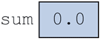
\includegraphics[width=\maxwidth,height=\maxheight,width=0.9\linewidth]{Figures/img_p254_0.png}
\end{center}

Ở lần thực thi đầu tiên của vòng lặp \texttt{for}, chúng ta đọc một giá
trị \texttt{3.2} từ người dùng và cộng giá trị này vào \texttt{sum}:

\begin{center}
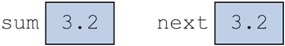
\includegraphics[width=\maxwidth,height=\maxheight,width=0.9\linewidth]{Figures/img_p254_1.png}
\end{center}

Lần thứ hai qua vòng lặp, chúng ta đọc một giá trị \texttt{4.7} và cộng
vào giá trị của \texttt{sum}:

\begin{center}
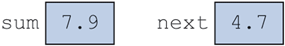
\includegraphics[width=\maxwidth,height=\maxheight,width=0.9\linewidth]{Figures/img_p254_2.png}
\end{center}

Lưu ý rằng \texttt{sum} hiện đã bao gồm cả hai số mà người dùng đã nhập,
vì chúng ta đã cộng giá trị mới, \texttt{4.7}, vào giá trị cũ,
\texttt{3.2}. Lần thứ ba qua vòng lặp, chúng ta cộng giá trị
\texttt{5.1}:

\begin{center}
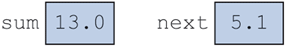
\includegraphics[width=\maxwidth,height=\maxheight,width=0.9\linewidth]{Figures/img_p254_3.png}
\end{center}

Lưu ý rằng biến \texttt{sum} hiện chứa tổng của ba số đầu tiên
(\texttt{3.2\ +\ 4.7\ +\ 5.1}). Bây giờ chúng ta đọc vào \texttt{9.0} và
cộng nó vào tổng:

\begin{center}
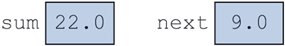
\includegraphics[width=\maxwidth,height=\maxheight,width=0.9\linewidth]{Figures/img_p255_0.png}
\end{center}

Sau đó, chúng ta cộng giá trị thứ năm, \texttt{2.4}:

\begin{center}
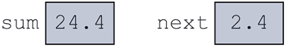
\includegraphics[width=\maxwidth,height=\maxheight,width=0.9\linewidth]{Figures/img_p255_1.png}
\end{center}

Cuối cùng, chúng ta cộng giá trị thứ sáu, \texttt{3.1}:

\begin{center}
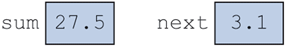
\includegraphics[width=\maxwidth,height=\maxheight,width=0.9\linewidth]{Figures/img_p255_2.png}
\end{center}

Sau đó, chúng ta thoát khỏi vòng lặp \texttt{for} và in ra giá trị của
\texttt{sum}.

Có một vấn đề phạm vi (scope) thú vị trong chương trình cụ thể này. Lưu
ý rằng biến \texttt{sum} được khai báo bên ngoài vòng lặp, trong khi
biến \texttt{next} được khai báo bên trong vòng lặp. Chúng ta không có
lựa chọn nào khác ngoài việc khai báo \texttt{sum} bên ngoài vòng lặp vì
nó cần được khởi tạo và nó được sử dụng sau vòng lặp. Nhưng biến
\texttt{next} chỉ được sử dụng bên trong vòng lặp, vì vậy nó có thể được
khai báo trong phạm vi bên trong đó. Tốt nhất là khai báo các biến trong
phạm vi trong cùng (innermost scope) có thể.

Thuật toán tính tổng tích lũy và các biến thể của nó sẽ hữu ích trong
nhiều tác vụ lập trình mà bạn giải quyết. Làm thế nào bạn có thể thực
hiện một phép tính tích tích lũy (cumulative product)? Đây là mã giả:

\begin{verbatim}
product = 1.
for (tất cả các số cần nhân) {
    lấy "next".
    product = product * next.
}
\end{verbatim}

\subsubsection{Vòng lặp tìm
Min/Max}\label{vuxf2ng-lux1eb7p-tuxecm-minmax}

Một tác vụ lập trình phổ biến khác là theo dõi các giá trị lớn nhất
và/hoặc nhỏ nhất trong một chuỗi. Ví dụ, hãy xem xét tác vụ quyết định
xem liệu có khả thi để xây dựng một khu vực sống trên Mặt trăng cho con
người ở hay không. Một trở ngại là nhiệt độ bề mặt trung bình hàng ngày
trên Mặt trăng là một mức lạnh giá -50 độ Fahrenheit. Nhưng một vấn đề
khó khăn hơn nhiều là phạm vi giá trị rộng; nó dao động từ mức tối thiểu
là -240 độ đến tối đa là 250 độ.

Để tính toán giá trị lớn nhất của một chuỗi các giá trị, bạn có thể theo
dõi giá trị lớn nhất mà bạn đã thấy cho đến nay và sử dụng lệnh
\texttt{if} để cập nhật giá trị lớn nhất nếu bạn bắt gặp một giá trị mới
lớn hơn giá trị lớn nhất hiện tại. Cách tiếp cận này có thể được mô tả
bằng mã giả như sau:

\begin{verbatim}
khởi tạo max.
for (tất cả các số cần kiểm tra) {
     lấy "next".
     if (next > max) {
        max = next.
    }
}
\end{verbatim}

Việc khởi tạo giá trị lớn nhất không hề đơn giản như bạn tưởng. Ví dụ,
những người mới học thường khởi tạo \texttt{max} thành \texttt{0}. Nhưng
chuyện gì sẽ xảy ra nếu chuỗi số mà bạn đang kiểm tra hoàn toàn bao gồm
các số âm? Ví dụ, bạn có thể được yêu cầu tìm giá trị lớn nhất của chuỗi
này:

-84, -7, -14, -39, -410, -17, -41, -9

Giá trị lớn nhất trong chuỗi này là -7 nhưng nếu bạn đã khởi tạo
\texttt{max} thành \texttt{0}, chương trình sẽ báo cáo không chính xác
\texttt{0} là giá trị lớn nhất.

Có hai giải pháp kinh điển cho vấn đề này. Đầu tiên, nếu bạn biết phạm
vi của các số bạn đang kiểm tra, bạn có thể đưa ra lựa chọn thích hợp
cho \texttt{max}. Trong trường hợp đó, bạn có thể đặt \texttt{max} thành
giá trị thấp nhất trong phạm vi. Điều đó có vẻ phản trực giác vì thông
thường chúng ta nghĩ giá trị lớn nhất là lớn, nhưng ý tưởng là đặt
\texttt{max} thành giá trị nhỏ nhất có thể để bất kỳ thứ gì lớn hơn sẽ
khiến \texttt{max} được đặt lại thành giá trị đó. Ví dụ, nếu bạn biết
rằng chuỗi nhiệt độ trước đó bao gồm các độ Fahrenheit, bạn sẽ biết rằng
nhiệt độ không bao giờ có thể nhỏ hơn độ không tuyệt đối (khoảng -460 độ
Fahrenheit), vì vậy bạn có thể khởi tạo \texttt{max} thành giá trị đó.

Khả năng thứ hai là khởi tạo \texttt{max} thành giá trị đầu tiên trong
chuỗi. Điều đó sẽ không phải lúc nào cũng thuận tiện vì nó có nghĩa là
phải lấy một trong các số bên ngoài vòng lặp.

Khi bạn kết hợp hai khả năng này, mã giả sẽ trở thành:

\begin{verbatim}
khởi tạo max bằng giá trị thấp nhất có thể hoặc bằng giá trị đầu tiên.
for (tất cả các số cần kiểm tra) {
    lấy "next".
    if (next > max) {
         max = next;
    }
}
\end{verbatim}

Mã giả để tính toán giá trị nhỏ nhất là một biến thể nhỏ của đoạn mã
này:

\begin{verbatim}
khởi tạo min bằng giá trị cao nhất có thể hoặc bằng giá trị đầu tiên.
for (tất cả các số cần kiểm tra) {
     lấy "next".
     if (next < min) {
         min = next.
    }
}
\end{verbatim}

Để giúp bạn hiểu rõ hơn về điều này, hãy đưa mã giả vào hành động với
một bài toán thực tế. Trong toán học, có một bài toán mở liên quan đến
những gì được gọi là dãy mưa đá (hailstone sequences). Các chuỗi số này
thường tăng và giảm theo các mô hình không thể đoán trước, hơi giống với
quá trình hình thành mưa đá. Một chuỗi mưa đá là một chuỗi các số trong
đó mỗi giá trị \(x\) được theo sau bởi:

\(3x + 1\), nếu \(x\) là số lẻ \(x / 2\), nếu \(x\) là số chẵn

Ví dụ, nếu bạn bắt đầu với 7 và tạo ra một chuỗi có độ dài 10, bạn sẽ
nhận được chuỗi: 7, 22, 11, 34, 17, 52, 26, 13, 40, 20 Trong chuỗi này,
giá trị lớn nhất và nhỏ nhất lần lượt là 52 và 7. Nếu bạn mở rộng phép
tính này cho một chuỗi có độ dài 20, bạn sẽ nhận được chuỗi: 7, 22, 11,
34, 17, 52, 26, 13, 40, 20, 10, 5, 16, 8, 4, 2, 1, 4, 2, 1 Trong trường
hợp này, giá trị lớn nhất và nhỏ nhất lần lượt là 52 và 1.

Bạn sẽ nhận thấy rằng một khi 1, 2, hoặc 4 xuất hiện trong chuỗi, chuỗi
sẽ tự lặp lại. Có giả thuyết cho rằng tất cả các số nguyên cuối cùng đều
đạt đến 1, giống như những hạt mưa đá rơi xuống đất. Đây là một bài toán
chưa có lời giải trong toán học. Không ai có thể bác bỏ nó, nhưng cũng
không ai chứng minh được nó.

Hãy viết một phương thức lấy một giá trị bắt đầu và độ dài chuỗi và in
ra giá trị lớn nhất và nhỏ nhất thu được trong một chuỗi mưa đá được tạo
bởi giá trị bắt đầu đó và có độ dài đó. Phương thức của chúng ta sẽ
trông như thế này:

\begin{verbatim}
public static void printHailstoneMaxMin(int value, int length) {
    ...
}
\end{verbatim}

Chúng ta có thể sử dụng giá trị bắt đầu để khởi tạo \texttt{max} và
\texttt{min}:

\begin{verbatim}
int min = value;
int max = value;
\end{verbatim}

Sau đó, chúng ta cần một vòng lặp sẽ tạo ra các giá trị khác. Lời gọi
phương thức sẽ cung cấp một giá trị cho tham số \texttt{length} cho
chúng ta biết số lần phải lặp qua vòng lặp, nhưng chúng ta không muốn
thực thi phần thân vòng lặp số lần bằng \texttt{length}: Hãy nhớ rằng
giá trị bắt đầu là một phần của chuỗi, vì vậy nếu chúng ta muốn sử dụng
một chuỗi có độ dài đã cho, chúng ta phải đảm bảo rằng số vòng lặp ít
hơn độ dài một đơn vị. Kết hợp ý tưởng này với mã giả
\texttt{max}/\texttt{min}, chúng ta biết vòng lặp sẽ trông như thế này:

\begin{verbatim}
for (int i = 1; i <= length - 1; i++) {
    tính số tiếp theo.
    if (value > max) {
         max = value.
    } else if (value < min) {
         min = value.
    }
}
in max và min.
\end{verbatim}

Để điền vào mã giả cho ``tính số tiếp theo'', chúng ta cần dịch công
thức toán học mưa đá sang mã. Công thức này khác nhau, tùy thuộc vào
việc giá trị hiện tại là lẻ hay chẵn. Chúng ta có thể sử dụng lệnh
\texttt{if/else} để giải quyết tác vụ này. Đối với biểu thức kiểm tra,
chúng ta có thể sử dụng phép kiểm tra ``mod 2'' để xem chúng ta nhận
được phần dư là bao nhiêu khi chia cho 2. Số chẵn có phần dư là 0 và số
lẻ có phần dư là 1. Vì vậy, biểu thức kiểm tra sẽ trông như thế này:

\begin{verbatim}
if (value % 2 == 0) {
    thực hiện phép tính chẵn.
} else {
    thực hiện phép tính lẻ.
}
\end{verbatim}

Dịch các công thức toán học mưa đá sang Java, chúng ta nhận được đoạn mã
sau:

\begin{verbatim}
if (value % 2 == 0) {
    value = value / 2;
} else {
    value = 3 * value + 1;
}
\end{verbatim}

Phần duy nhất trong mã giả của chúng ta mà chúng ta chưa điền là phần in
ra kết quả. Phần này diễn ra sau vòng lặp và khá dễ hoàn thành. Đây là
phương thức hoàn chỉnh:

\begin{verbatim}
public static void printHailstoneMaxMin(int value, int length) {
    int min = value;
    int max = value;
  for (int i = 1; i <= length - 1; i++) {
      if (value % 2 == 0) {
          value = value / 2;
      } else {
          value = 3 * value + 1;
      }
      if (value > max) {
          max = value;
      } else if (value < min) {
          min = value;
      }
  }
  System.out.println("max = " + max);
  System.out.println("min = " + min);
}
\end{verbatim}

\subsubsection{Tính tổng tích lũy với
if}\label{tuxednh-tux1ed5ng-tuxedch-lux169y-vux1edbi-if}

Bây giờ chúng ta hãy khám phá cách bạn có thể sử dụng các lệnh
\texttt{if/else} để tạo ra một số biến thể thú vị trên thuật toán tính
tổng tích lũy.

Giả sử bạn muốn đọc một chuỗi số và tính trung bình. Tác vụ này có vẻ
giống như một biến thể đơn giản của mã tính tổng tích lũy. Bạn có thể
tính trung bình bằng tổng chia cho số lượng số:

\begin{verbatim}
double average = sum / totalNumber;
System.out.println("average = " + average);
\end{verbatim}

Nhưng có một vấn đề nhỏ với đoạn mã này. Giả sử rằng khi chương trình
hỏi người dùng số lượng số cần xử lý, người dùng nhập \texttt{0}. Sau đó
chương trình sẽ không vào vòng lặp tính tổng tích lũy và mã của bạn sẽ
cố gắng tính giá trị của \texttt{0} chia cho \texttt{0}. Java sau đó sẽ
in ra trung bình là \texttt{NaN}, một thông báo khó hiểu viết tắt của
``Not a Number''. Sẽ tốt hơn nếu chương trình in ra một loại thông báo
khác cho biết không có số nào để tính trung bình. Bạn có thể sử dụng một
lệnh \texttt{if/else} cho mục đích này:

\begin{verbatim}
if (totalNumber <= 0) {
    System.out.println("No numbers to average");
} else {
    double average = sum / totalNumber;
    System.out.println("average = " + average);
}
\end{verbatim}

Một cách sử dụng khác của lệnh \texttt{if} sẽ là đếm số lượng số âm mà
người dùng nhập vào. Bạn sẽ thường muốn đếm số lần một điều gì đó xảy ra
trong chương trình. Mục tiêu này dễ dàng đạt được với một lệnh
\texttt{if} và một biến số nguyên được gọi là bộ đếm (counter). Bạn bắt
đầu bằng cách khởi tạo bộ đếm thành \texttt{0}:

\begin{verbatim}
int negatives = 0;
\end{verbatim}

Bạn có thể sử dụng bất kỳ tên nào bạn muốn cho biến. Ở đây chúng tôi sử
dụng \texttt{negatives} bởi vì đó là những gì bạn đang đếm. Bước cần
thiết khác là tăng bộ đếm bên trong vòng lặp nếu nó vượt qua bài kiểm
tra đang được quan tâm:

\begin{verbatim}
if (next < 0) {
    negatives++;
}
\end{verbatim}

Khi bạn kết hợp tất cả những điều này lại với nhau và sửa đổi các chú
thích cũng như phần giới thiệu, bạn sẽ có biến thể sau của chương trình
tính tổng tích lũy:

\begin{verbatim}
 1 // Finds the average of a sequence of numbers as well as
 2 // reporting how many of the user-specified numbers were negative.
 3
 4 import java.util.*;
 5
 6 public class ExamineNumbers2 {
 7     public static void main(String[] args) {
 8         System.out.println("This program examines a sequence");
 9         System.out.println("of numbers to find the average");
10         System.out.println("and count how many are negative.");
\end{verbatim}

\begin{verbatim}
           negatives++;
        }
    }
    System.out.println();

    if (totalNumber <= 0) {
       System.out.println("No numbers to average");
   } else {
       double average = sum / totalNumber;
       System.out.println("average = " + average);
   }
   System.out.println("# of negatives = " + negatives);
 }
}
\end{verbatim}

Quá trình thực thi của chương trình sẽ trông giống như thế này:

\begin{verbatim}
This program examines a sequence 
of numbers to find the average 
and count how many are negative. 
 
How many numbers do you have? 8  
    #1? 2.5  
    #2? 9.2  
    #3? -19.4  
    #4? 208.2  
    #5? 42.3  
    #6? 92.7  
    #7? -17.4  
    #8? 8  
average = 40.7625 
# of negatives = 2
\end{verbatim}

\subsubsection{Sai số làm tròn (Roundoff
Errors)}\label{sai-sux1ed1-luxe0m-truxf2n-roundoff-errors}

Khi bạn khám phá các thuật toán tích lũy, bạn sẽ phát hiện ra một vấn đề
cụ thể mà bạn nên hiểu. Ví dụ, hãy xem xét lần thực thi sau của chương
trình \texttt{ExamineNumbers2} trước đó với dữ liệu đầu vào khác của
người dùng:

\begin{verbatim}
This program examines a sequence 
of numbers to find the average 
and count how many are negative. 
 
How many numbers do you have? 4 
    #1? 2.1  
    #2? -3.8  
    #3? 5.4  
    #4? 7.4  
average = 2.7750000000000004 
# of negatives = 1
\end{verbatim}

Nếu bạn sử dụng máy tính, bạn sẽ thấy rằng bốn số cộng lại bằng 11.1.
Nếu bạn chia số này cho 4, bạn sẽ nhận được 2.775. Tuy nhiên, Java báo
cáo kết quả là \texttt{2.7750000000000004}. Tất cả những số 0 đó từ đâu
ra và tại sao số đó lại kết thúc bằng số 4? Câu trả lời là các số dấu
phẩy động (floating-point numbers) có thể dẫn đến sai số làm tròn
(roundoff errors).

\begin{quote}
\textbf{Sai số làm tròn (Roundoff Error)} Lỗi số học xảy ra do các số
dấu phẩy động được lưu trữ dưới dạng giá trị gần đúng chứ không phải là
giá trị chính xác.
\end{quote}

Các sai số làm tròn nhìn chung là nhỏ và có thể xảy ra theo một trong
hai hướng (hơi cao hoặc hơi thấp). Trong trường hợp trước, chúng ta gặp
sai số làm tròn hơi cao.

Các số dấu phẩy động được lưu trữ ở định dạng tương tự như ký hiệu khoa
học (scientific notation), với một tập hợp các chữ số và một số mũ
(exponent). Hãy xem xét cách bạn sẽ lưu trữ giá trị một phần ba bằng ký
hiệu khoa học ở cơ số 10. Bạn sẽ nói rằng số đó là 3.33333 (lặp lại)
nhân với 10 lũy thừa -1. Tuy nhiên, chúng ta không thể lưu trữ vô số chữ
số trên máy tính, vì vậy chúng ta sẽ phải ngừng lặp lại số 3 ở một thời
điểm nào đó. Giả sử chúng ta có thể lưu trữ 10 chữ số. Khi đó, giá trị
của một phần ba sẽ được lưu trữ là 3.333333333 nhân với 10 lũy thừa -1.
Nếu chúng ta nhân số đó với 3, chúng ta không nhận lại được 1. Thay vào
đó, chúng ta nhận được 9.999999999 nhân với 10 lũy thừa -1 (tương đương
với 0.9999999999).

Bạn có thể thắc mắc tại sao các số chúng ta sử dụng trong ví dụ trước
lại gây ra sự cố khi chúng không có bất kỳ chữ số lặp lại nào. Bạn phải
nhớ rằng máy tính lưu trữ các số ở cơ số 2. Các số như 2.1 và 5.4 có thể
trông giống như các số đơn giản ở cơ số 10, nhưng chúng có các chữ số
lặp lại khi được lưu trữ ở cơ số 2.

Sai số làm tròn có thể dẫn đến những kết quả khá bất ngờ. Ví dụ, hãy xem
xét chương trình ngắn sau đây:

\begin{verbatim}
 1 // This program demonstrates roundoff errors.
 2 public class Roundoff {
 3     public static void main(String[] args) {
 4         double n = 1.0;
 5         for (int i = 1; i <= 10; i++) {
 6              n += 0.1;
 7             System.out.println(n);
 8         }
 9     }
10 }
\end{verbatim}

Chương trình này trình bày một phép tính tổng tích lũy cổ điển với một
vòng lặp cộng thêm \texttt{0.1} vào biến \texttt{n} mỗi lần vòng lặp
thực thi. Chúng ta bắt đầu với \texttt{n} bằng \texttt{1.0} và vòng lặp
lặp lại 10 lần, điều mà chúng ta có thể mong đợi sẽ in ra các số 1.1,
1.2, 1.3 và vân vân cho đến 2.0. Thay vào đó, nó tạo ra kết quả sau:

\begin{verbatim}
1.1 
\end{verbatim}

\begin{verbatim}
1.2000000000000002 
1.3000000000000003 
1.4000000000000004 
1.5000000000000004 
1.6000000000000005 
1.7000000000000006 
1.8000000000000007 
1.9000000000000008 
2.000000000000001
\end{verbatim}

Vấn đề xảy ra vì 0.1 không thể được lưu trữ chính xác ở cơ số 2 (nó tạo
ra một tập hợp các chữ số lặp lại, giống như một phần ba ở cơ số 10).
Mỗi lần lặp qua vòng lặp, lỗi lại được cộng dồn, đó là lý do tại sao sai
số làm tròn lại trở nên tồi tệ hơn sau mỗi lần lặp.

Như một ví dụ khác, hãy xem xét tác vụ cộng các giá trị của một đồng xu
một xu, một đồng 5 xu, một đồng 10 xu và một đồng 25 xu. Nếu chúng ta sử
dụng các biến kiểu \texttt{int}, chúng ta sẽ nhận được câu trả lời chính
xác bất kể thứ tự mà chúng ta cộng các số:

\begin{verbatim}
jshell> int cents1 = 1 + 5 + 10 + 25; 
cents1 ==> 41
jshell> int cents2 = 25 + 10 + 5 + 1; 
cents2 ==> 41
\end{verbatim}

Bất kể thứ tự như thế nào, các con số này luôn cộng lại bằng 41 xu.
Nhưng giả sử thay vì nghĩ về các giá trị này là toàn bộ số xu, chúng ta
nghĩ về chúng như một phần nhỏ của đồng đô la mà chúng ta lưu trữ dưới
dạng \texttt{double}:

\begin{verbatim}
jshell> double dollars1 = 0.01 + 0.05 + 0.10 + 0.25; 
dollars1 ==> 0.41000000000000003
jshell> double dollars2 = 0.25 + 0.10 + 0.05 + 0.01; 
dollars2 ==> 0.41
\end{verbatim}

Mặc dù chúng ta cộng chính xác cùng những con số, thực tế là chúng ta
cộng chúng theo một thứ tự khác lại tạo ra sự khác biệt. Lý do là sai số
làm tròn.

Có một số bài học cần rút ra từ điều này: - Hãy nhận biết rằng khi bạn
lưu trữ các giá trị dấu phẩy động (ví dụ: \texttt{double}), bạn đang lưu
trữ các giá trị gần đúng chứ không phải là các giá trị chính xác. Nếu
bạn cần lưu trữ một giá trị chính xác, hãy lưu trữ nó bằng kiểu
\texttt{int}. - Đừng ngạc nhiên khi bạn thấy các con số hơi khác so với
các giá trị dự kiến. - Đừng mong đợi có thể so sánh các biến kiểu
\texttt{double} để kiểm tra sự bằng nhau.

Để theo dõi ý thứ ba, hãy xem xét đoạn mã trước đó sẽ dẫn đến điều gì
nếu chúng ta thực hiện biểu thức kiểm tra sau:

\begin{verbatim}
if (dollars1 == dollars2) {
   ...
}
\end{verbatim}

Biểu thức kiểm tra sẽ đánh giá thành \texttt{false} bởi vì các giá trị
rất gần nhau, nhưng không đủ gần để Java coi chúng là bằng nhau. Chúng
ta hiếm khi sử dụng bài kiểm tra về sự bằng nhau chính xác khi làm việc
với \texttt{double}. Thay vào đó, chúng ta có thể sử dụng một biểu thức
kiểm tra như thế này để xem liệu các số có gần bằng nhau không:

\begin{verbatim}
if (Math.abs(dollars1 - dollars2) < 0.001) {
   ...
}
\end{verbatim}

Chúng ta sử dụng phương thức giá trị tuyệt đối (\texttt{abs}) từ lớp
\texttt{Math} để tìm độ lớn của phần chênh lệch và sau đó kiểm tra xem
nó có nhỏ hơn một lượng nhỏ nào đó không (trong trường hợp này là
\texttt{0.001}).

Phần sau trong chương này, chúng tôi sẽ giới thiệu một biến thể của
\texttt{print}/\texttt{println} được gọi là \texttt{printf} sẽ giúp việc
in các số như thế này mà không có tất cả các chữ số thừa dễ dàng hơn.

\subsection{Xử lý văn bản (Text
Processing)}\label{xux1eed-luxfd-vux103n-bux1ea3n-text-processing-1}

Các lập trình viên thường phải đối mặt với các bài toán yêu cầu họ phải
tạo, chỉnh sửa, kiểm tra và định dạng văn bản. Nói chung, chúng tôi gọi
những tác vụ này là xử lý văn bản.

\begin{quote}
\textbf{Xử lý văn bản (Text Processing)} Chỉnh sửa và định dạng chuỗi
văn bản.
\end{quote}

Trong phần này, chúng ta sẽ xem xét chi tiết hơn về kiểu dữ liệu nguyên
thủy \texttt{char} và giới thiệu một lệnh mới được gọi là
\texttt{System.out.printf}. Cả hai công cụ này đều rất hữu ích cho các
tác vụ xử lý văn bản.

\subsubsection{Kiểu char}\label{kiux1ec3u-char}

Kiểu dữ liệu nguyên thủy \texttt{char} đại diện cho một ký tự văn bản
duy nhất. Việc có các biến, tham số và giá trị trả về có kiểu
\texttt{char} là hoàn toàn hợp lệ nếu bạn muốn. Các giá trị nghĩa đen
(literal values) của kiểu \texttt{char} được biểu thị bằng cách đặt ký
tự bên trong dấu nháy đơn:

\begin{verbatim}
char ch = 'A';
\end{verbatim}

Bạn cũng có thể tạo giá trị \texttt{char} đại diện cho một chuỗi thoát
(escape sequence):

\begin{verbatim}
char newline = '\n';
\end{verbatim}

Trong chương trước, chúng ta đã thảo luận về các đối tượng
\texttt{String}. Sự khác biệt giữa \texttt{char} và \texttt{String} là
một sự khác biệt tinh tế khiến nhiều lập trình viên Java mới bối rối. Sự
khác biệt chính là \texttt{String} là một đối tượng, nhưng \texttt{char}
là một giá trị nguyên thủy. Một \texttt{char} chiếm một dung lượng bộ
nhớ rất nhỏ, nhưng nó không có các phương thức. Bảng 4.4 tóm tắt một số
khác biệt giữa các kiểu.

Bảng 4.4 Sự khác biệt giữa \texttt{char} và \texttt{String}

\begin{center}

\includegraphics[width=\maxwidth,height=\maxheight,width=0.9\linewidth]{Figures/img_p275_0.png}
\end{center}

Tại sao Java lại có hai kiểu cho dữ liệu tương tự như vậy? Kiểu
\texttt{char} tồn tại chủ yếu vì những lý do lịch sử; nó có từ các ngôn
ngữ cũ hơn như C, ngôn ngữ đã ảnh hưởng đến thiết kế của Java.

Vậy tại sao một người lại sử dụng kiểu \texttt{char} khi \texttt{String}
có sẵn? Việc sử dụng \texttt{char} thường là cần thiết vì một số phương
thức trong API của Java sử dụng nó làm kiểu tham số hoặc kiểu trả về.
Nhưng cũng có

một vài trường hợp mà việc sử dụng \texttt{char} có thể hữu ích hoặc đơn
giản hơn việc sử dụng \texttt{String}.

Các ký tự của một \texttt{String} được lưu trữ bên trong đối tượng dưới
dạng các giá trị kiểu \texttt{char}. Bạn có thể truy cập các ký tự riêng
lẻ thông qua phương thức \texttt{charAt} của đối tượng, phương thức này
nhận một chỉ số nguyên làm tham số và trả về ký tự tại chỉ số đó. Chúng
ta thường lặp qua một chuỗi để kiểm tra hoặc thay đổi các ký tự của nó.
Ví dụ, phương thức sau in mỗi ký tự của một chuỗi trên một dòng riêng
của nó:

\begin{verbatim}
public static void printVertical(String message) {
    for (int i = 0; i < message.length(); i++) {
        char ch = message.charAt(i);
        System.out.println(ch);
    }
}
\end{verbatim}

\subsubsection{\texorpdfstring{\texttt{char} so với
\texttt{int}}{char so với int}}\label{char-so-vux1edbi-int}

Các giá trị kiểu \texttt{char} được lưu trữ nội bộ dưới dạng các số
nguyên. Một sơ đồ mã hóa tiêu chuẩn được gọi là Unicode xác định giá trị
số nguyên nào đại diện cho mỗi ký tự. (Unicode sẽ được đề cập chi tiết
hơn ở phần sau của chương này.) Vì các ký tự thực chất là các số nguyên,
Java sẽ tự động chuyển đổi giá trị kiểu \texttt{char} thành \texttt{int}
bất cứ khi nào nó mong đợi một \texttt{int}:

\begin{verbatim}
int letter = 'a' + 2; // stores 99
\end{verbatim}

Hóa ra giá trị số nguyên của
\texttt{\textquotesingle{}a\textquotesingle{}} là \texttt{97}, vì vậy
kết quả của biểu thức là \texttt{99}, được lưu trữ dưới dạng ký tự
\texttt{\textquotesingle{}c\textquotesingle{}}. Tương tự, một
\texttt{int} có thể được chuyển đổi thành một \texttt{char} bằng cách sử
dụng ép kiểu (type cast). (Việc ép kiểu là cần thiết như một lời hứa với
trình biên dịch, vì không phải mọi giá trị \texttt{int} có thể đều tương
ứng với một ký tự hợp lệ.) Dưới đây là ví dụ về một đoạn mã sử dụng ép
kiểu để chuyển đổi giá trị \texttt{int} thành giá trị kiểu
\texttt{char}:

\begin{verbatim}
int code = 66;
char grade = (char) code; // stores 'B'
\end{verbatim}

Vì các giá trị kiểu \texttt{char} thực chất là các số nguyên, chúng cũng
có thể được so sánh bằng các toán tử quan hệ như \texttt{\textless{}}
hoặc \texttt{==}. Ngoài ra, chúng có thể được sử dụng trong các vòng lặp
để bao phủ các phạm vi chữ cái. Ví dụ, đoạn mã sau in ra mọi chữ cái của
bảng chữ cái:

\begin{verbatim}
for (char letter = 'a'; letter <= 'z'; letter++) {
    System.out.print(letter);
}
\end{verbatim}

\begin{verbatim}
if (grade == 'B') {... // true
\end{verbatim}

Bạn có thể tìm hiểu thêm về sự tương đương giữa ký tự và số nguyên bằng
cách tìm kiếm trên web các bảng Unicode.

\subsubsection{Các thuật toán văn bản tích lũy (Cumulative Text
Algorithms)}\label{cuxe1c-thuux1eadt-touxe1n-vux103n-bux1ea3n-tuxedch-lux169y-cumulative-text-algorithms}

Các chuỗi ký tự thường được sử dụng trong các thuật toán tích lũy như đã
thảo luận ở phần trước trong chương này. Ví dụ, bạn có thể lặp qua các
ký tự của một chuỗi để tìm kiếm một chữ cái cụ thể. Phương thức sau chấp
nhận một chuỗi và một ký tự và trả về số lần ký tự đó xuất hiện trong
chuỗi:

\begin{verbatim}
public static int count(String text, char c) {
    int found = 0;
    for (int i = 0; i < text.length(); i++) {
        if (text.charAt(i) == c) {
            found++;
        }
    }
    return found;
}
\end{verbatim}

Một \texttt{char} có thể được ghép với một \texttt{String} bằng cách sử
dụng toán tử \texttt{+} tiêu chuẩn. Sử dụng ý tưởng này, một
\texttt{String} có thể được xây dựng bằng một vòng lặp, bắt đầu với một
chuỗi rỗng và ghép các ký tự riêng lẻ trong vòng lặp. Đây được gọi là
phép nối tích lũy (cumulative concatenation). Phương thức sau chấp nhận
một chuỗi và trả về các ký tự tương tự theo thứ tự ngược lại:

\begin{verbatim}
public static String reverse(String phrase) {
    String result = "";
    for (int i = 0; i < phrase.length(); i++) {
         result = phrase.charAt(i) + result;
    }
    return result;
}
\end{verbatim}

Ví dụ, lệnh gọi \texttt{reverse("Tin\ man\ ")} trả về
\texttt{"nam\ niT"}.

Vì \texttt{char} là một kiểu dữ liệu nguyên thủy, bạn không thể sử dụng
cú pháp dấu chấm để gọi các phương thức như cách bạn làm với một giá trị
kiểu \texttt{String}. Thay vào đó, Java cung cấp một lớp gọi là
\texttt{Character} có một số phương thức tĩnh (static methods) cho phép
bạn xác minh xem bạn có loại ký tự nào (chữ số, chữ cái, v.v.) và thực
hiện nhiều chuyển đổi khác nhau. Một số phương thức \texttt{Character}
hữu ích nhất được liệt kê trong Bảng 4.5.

Bảng 4.5 Các phương thức hữu ích của lớp \texttt{Character}

\begin{center}

\includegraphics[width=\maxwidth,height=\maxheight,width=0.9\linewidth]{Figures/img_p279_0.png}
\end{center}

Phương thức sau đếm số lượng chữ cái trong một \texttt{String}, bỏ qua
tất cả các ký tự không phải chữ cái như dấu câu, số và khoảng trắng:

\begin{verbatim}
public static int countLetters(String phrase) {
    int count = 0;
    for (int i = 0; i < phrase.length(); i++) {
        char ch = phrase.charAt(i);
          if (Character.isLetter(ch)) {
              count++;
        }
    }
    return count;
}
\end{verbatim}

Ví dụ, lệnh gọi \texttt{countLetters("gr8\ JoB!\ ")} trả về 5.

\subsubsection{System.out.printf}\label{system.out.printf}

Cho đến nay, chúng ta đã sử dụng \texttt{System.out.println} và
\texttt{System.out.print} cho đầu ra của bảng điều khiển (console
output). Có một phương thức thứ ba, \texttt{System.out.printf}, phức tạp
hơn một chút so với các phương thức khác nhưng cung cấp cho chúng ta một
số khả năng mới hữu ích. Chữ ``f'' trong \texttt{printf} là viết tắt của
``formatted'', ngụ ý rằng \texttt{System.out.printf} cung cấp cho bạn
nhiều quyền kiểm soát hơn đối với định dạng mà đầu ra của bạn được in
ra.

Hãy tưởng tượng rằng bạn muốn in một bảng cửu chương từ 1 đến 10. Đoạn
mã sau in ra các số chính xác, nhưng nó trông không được đẹp cho lắm:

\begin{verbatim}
for (int i = 1; i <= 10; i++) {
    for (int j = 1; j <= 10; j++) {
        System.out.print(i * j + " ");
    }
    System.out.println();
}
\end{verbatim}

Đầu ra là như sau. Lưu ý rằng các số không thẳng hàng theo chiều dọc:

\begin{verbatim}
1 2 3 4 5 6 7 8 9 10 
2 4 6 8 10 12 14 16 18 20 
3 6 9 12 15 18 21 24 27 30 
4 8 12 16 20 24 28 32 36 40 
5 10 15 20 25 30 35 40 45 50 
6 12 18 24 30 36 42 48 54 60 
7 14 21 28 35 42 49 56 63 70 
8 16 24 32 40 48 56 64 72 80 
9 18 27 36 45 54 63 72 81 90 
10 20 30 40 50 60 70 80 90 100
\end{verbatim}

Chúng ta có thể phân tách các số bằng các tab, điều này sẽ tốt hơn.
Nhưng sự phân tách này không cho chúng ta nhiều quyền kiểm soát đối với
giao diện của bảng. Mỗi số sẽ cách nhau chính xác tám khoảng trắng trên
màn hình và các số sẽ xuất hiện căn trái. Sẽ rất phiền phức nếu cố gắng
căn phải các số một cách thủ công, bởi vì bạn sẽ phải sử dụng các lệnh
\texttt{if/else} để kiểm tra xem một số cụ thể có nằm trong một phạm vi
nhất định hay không và, nếu cần, đệm nó với một số lượng khoảng trắng
nhất định.

\begin{quote}
\textbf{BẠN CÓ BIẾT?} \textbf{ASCII và Unicode} Chúng ta lưu trữ dữ liệu
trên máy tính dưới dạng số nhị phân (các chuỗi số 0 và 1). Để lưu trữ dữ
liệu văn bản, chúng ta cần một sơ đồ mã hóa cho chúng ta biết nên sử
dụng chuỗi số 0 và 1 nào cho bất kỳ ký tự nhất định nào. Hãy coi nó như
một chiếc nhẫn giải mã bí mật khổng lồ cho biết những điều như, ``Nếu
bạn muốn lưu trữ một chữ `a' thường, hãy sử dụng chuỗi 01100001.'' Đầu
những năm 1960, IBM đã phát triển một sơ đồ mã hóa gọi là EBCDIC hoạt
động tốt với các thẻ đục lỗ của công ty, thứ đã được sử dụng trong nhiều
thập kỷ trước khi máy tính được phát minh. Nhưng chẳng bao lâu sau, rõ
ràng EBCDIC không phải là một sơ đồ mã hóa thuận tiện cho các lập trình
viên máy tính. Có những khoảng trống trong chuỗi làm cho các ký tự như
`i' và `j' xuất hiện cách xa nhau mặc dù chúng đứng ngay sau nhau. Năm
1967, Hiệp hội Tiêu chuẩn Hoa Kỳ (American Standards Association) đã
công bố một sơ đồ được gọi là ASCII (phát âm là ``AS-kee'') được sử dụng
phổ biến kể từ đó. Tên viết tắt này là viết tắt của ``American Standard
Code for Information Interchange'' (Mã chuẩn Hoa Kỳ về trao đổi thông
tin). Ở dạng ban đầu, ASCII định nghĩa 128 ký tự, mỗi ký tự có thể được
lưu trữ với 7 bit dữ liệu. Vấn đề lớn nhất với ASCII là nó là một mã của
Mỹ. Có rất nhiều ký tự được sử dụng phổ biến ở các quốc gia khác không
được bao gồm trong ASCII. Ví dụ, đồng bảng Anh (£) và biến thể tiếng Tây
Ban Nha của chữ n (ñ) không được bao gồm trong 128 ký tự ASCII tiêu
chuẩn. Đã có nhiều nỗ lực nhằm mở rộng ASCII, nhân đôi nó lên 256 ký tự
để nó có thể bao gồm nhiều ký tự đặc biệt này. Tuy nhiên, hóa ra ngay cả
256 ký tự cũng không đủ để nắm bắt sự đa dạng đáng kinh ngạc của giao
tiếp của con người. Khoảng thời gian Java được tạo ra, một liên minh của
các chuyên gia phần mềm đã giới thiệu một tiêu chuẩn mới để mã hóa các
ký tự được gọi là Unicode. Họ quyết định rằng 7 bit của ASCII tiêu chuẩn
và 8 bit của ASCII mở rộng đơn giản là không đủ lớn và quyết định không
đặt giới hạn về số lượng bit họ có thể sử dụng để mã hóa ký tự. Tại thời
điểm viết bài này, liên minh đã xác định được hơn 110,000 ký tự, yêu cầu
nhiều hơn 16 bit một chút để lưu trữ. Unicode bao gồm các ký tự được sử
dụng trong hầu hết các ngôn ngữ hiện đại và thậm chí cả một số ngôn ngữ
cổ đại. Chữ tượng hình Ai Cập đã được thêm vào năm 2007, mặc dù nó vẫn
không bao gồm chữ tượng hình của người Maya và liên minh đã từ chối một
đề xuất bao gồm các ký tự Klingon. Các nhà thiết kế của Java đã sử dụng
Unicode làm tiêu chuẩn cho kiểu \texttt{char}, điều đó có nghĩa là các
chương trình Java có khả năng thao tác với đầy đủ các ký tự. May mắn
thay, Liên minh Unicode đã quyết định kết hợp các bảng mã ASCII, vì vậy
ASCII có thể được xem như một tập con của Unicode. Nếu bạn tò mò về thứ
tự thực tế của các ký tự trong ASCII, hãy gõ ``bảng ASCII'' vào công cụ
tìm kiếm yêu thích của bạn và bạn sẽ tìm thấy hàng triệu lượt truy cập
để khám phá.
\end{quote}

Một cách dễ dàng hơn nhiều để in các giá trị được căn lề trong các
trường có độ rộng cố định là sử dụng lệnh \texttt{System.out.printf}.
Phương thức \texttt{printf} chấp nhận một \texttt{String} được viết đặc
biệt gọi là chuỗi định dạng (format string) chỉ định giao diện chung của
đầu ra, theo sau là bất kỳ tham số nào sẽ được bao gồm trong đầu ra:

\begin{verbatim}
System.out.printf(<format string>, <parameter>,..., <parameter>);
\end{verbatim}

Một chuỗi định dạng giống như một \texttt{String} bình thường, ngoại trừ
việc nó có thể chứa các chỗ dành sẵn (placeholders) được gọi là công cụ
xác định định dạng (format specifiers) cho phép bạn chỉ định một vị trí
mà giá trị của một biến sẽ được chèn vào, cùng với định dạng bạn muốn
cung cấp cho giá trị đó. Các công cụ xác định định dạng bắt đầu bằng dấu
\texttt{\%} và kết thúc bằng một chữ cái xác định loại giá trị, chẳng
hạn như \texttt{d} cho số nguyên thập phân (\texttt{int}) hoặc
\texttt{f} cho số dấu phẩy động (số thực kiểu \texttt{double}). Hãy xem
xét lệnh \texttt{printf} sau:

\begin{verbatim}
int x = 38, y = -152;
System.out.printf("location: (%d, %d)\n", x, y);
\end{verbatim}

Lệnh này tạo ra đầu ra sau:

\begin{verbatim}
location: (38, -152)
\end{verbatim}

Dấu \texttt{\%d} không thực sự được in ra mà thay vào đó được thay thế
bằng tham số tương ứng được viết sau chuỗi định dạng. Số lượng công cụ
xác định định dạng trong chuỗi định dạng phải khớp với số lượng tham số
theo sau nó. Công cụ xác định đầu tiên sẽ được thay thế bằng tham số đầu
tiên, công cụ xác định thứ hai bằng tham số thứ hai, và vân vân.
\texttt{System.out.printf} là bất thường vì nó có thể chấp nhận một số
lượng tham số thay đổi.

Lệnh \texttt{printf} giống như \texttt{System.out.print} ở chỗ nó không
di chuyển sang một dòng mới trừ khi bạn ra lệnh rõ ràng cho nó làm như
vậy. Lưu ý rằng trong đoạn mã trước, chúng ta đã kết thúc chuỗi định
dạng của mình bằng \texttt{\textbackslash{}n} để hoàn thành dòng đầu ra.

Vì một công cụ xác định định dạng sử dụng \texttt{\%} làm ký tự đặc
biệt, nếu bạn muốn in ký hiệu \texttt{\%} thực tế trong một lệnh
\texttt{printf}, thay vào đó hãy viết hai ký tự \texttt{\%} liên tiếp.
Ví dụ:

\begin{verbatim}
int score = 87;
System.out.printf("You got %d%% on the exam!\n", score);
\end{verbatim}

Mã tạo ra đầu ra sau:

\begin{verbatim}
You got 87% on the exam!
\end{verbatim}

Một công cụ xác định định dạng có thể chứa thông tin sau dấu \texttt{\%}
để chỉ định chiều rộng, độ chính xác và căn lề của giá trị đang được in.
Ví dụ, \texttt{\%8d} chỉ định một số nguyên căn phải trong một khu vực
rộng 8 khoảng trắng và \texttt{\%12.4f} chỉ định một giá trị
\texttt{double} căn phải trong một khu vực rộng 12 khoảng trắng, được
làm tròn đến bốn chữ số sau dấu thập phân. Bảng 4.6 liệt kê một số công
cụ xác định định dạng phổ biến mà bạn có thể muốn sử dụng trong các
chương trình của mình.

Bảng 4.6 Các công cụ xác định định dạng phổ biến

\begin{center}

\includegraphics[width=\maxwidth,height=\maxheight,width=0.9\linewidth]{Figures/img_p286_0.png}
\end{center}

Như một ví dụ toàn diện, giả sử rằng các biến sau đã được khai báo để
biểu thị thông tin về một học sinh:

\begin{verbatim}
int score = 87;
double gpa = 3.18652;
String name = "Jessica";
\end{verbatim}

Đoạn mã mẫu sau in các biến trước đó bằng một số công cụ xác định định
dạng:

\begin{verbatim}
System.out.printf("student name: %10s\n", name);
System.out.printf("exam score  : %10d\n", score);
System.out.printf("GPA       : %10.2f\n", gpa);
\end{verbatim}

Mã tạo ra đầu ra sau:

\begin{verbatim}
student name:     Jessica 
exam score  :          87 
GPA       :        3.19
\end{verbatim}

Ba giá trị thẳng hàng ở cạnh phải của chúng, bởi vì chúng ta in tất cả
chúng với chiều rộng bằng 10. Phương thức \texttt{printf} giúp việc sắp
xếp các giá trị thành các cột theo cách này trở nên dễ dàng. Lưu ý rằng
điểm trung bình (GPA) của học sinh làm tròn thành 3.19, do số \texttt{2}
trong công cụ xác định định dạng của biến đó. Công cụ xác định
\texttt{10.2} làm cho giá trị vừa khít với một khu vực rộng 10 ký tự với
chính xác 2 chữ số sau dấu thập phân.

Hãy quay lại ví dụ về bảng cửu chương của chúng ta. Bây giờ chúng ta đã
biết về \texttt{printf}, chúng ta có thể in bảng với các con số được căn
phải tương đối dễ dàng. Chúng ta sẽ căn phải các con số vào các trường
có chiều rộng 5:

\begin{verbatim}
for (int i = 1; i <= 10; i++) {
    for (int j = 1; j <= 10; j++) {
        System.out.printf("%5d", i * j); 
    }
    System.out.println();
}
\end{verbatim}

Đoạn mã này tạo ra đầu ra sau:

\begin{verbatim}
  1    2    3    4    5    6    7    8    9    10 
  2    4    6    8   10   12   14   16   18    20 
  3    6    9   12   15   18   21   24   27    30 
  4    8   12   16   20   24   28   32   36    40 
  5   10   15   20   25   30   35   40   45    50 
  6   12   18   24   30   36   42   48   54    60 
  7   14   21   28   35   42   49   56   63    70 
  8   16   24   32   40   48   56   64   72    80 
  9   18   27   36   45   54   63   72   81    90 
 10   20   30   40   50   60   70   80   90   100
\end{verbatim}

Phương thức \texttt{printf} cũng có thể giải quyết sự cố với chương
trình \texttt{Roundoff} được giới thiệu ở phần trước trong chương này.
Việc cố định độ chính xác của giá trị \texttt{double} đảm bảo rằng nó sẽ
được làm tròn để tránh những sai số làm tròn nhỏ xíu do số học
\texttt{double} mang lại. Đây là chương trình đã được sửa đổi:

\begin{verbatim}
  1 // Uses System.out.printf to correct roundoff errors.
  2 public class Roundoff2 {
  3     public static void main(String[] args) {
  4         double n = 1.0;
  5         for (int i = 1; i <= 10; i++) {
  6             n += 0.1;
  7              System.out.printf("%3.1f\n", n);
  8         }
  9     }
 10 }
\end{verbatim}

Chương trình tạo ra đầu ra sau:

\begin{verbatim}
1.1 
1.2 
1.3 
1.4 
1.5 
1.6 
1.7 
1.8 
1.9 
2.0
\end{verbatim}

\subsection{Phương thức với Thực thi có điều kiện (Methods with
Conditional
Execution)}\label{phux1b0ux1a1ng-thux1ee9c-vux1edbi-thux1ef1c-thi-cuxf3-ux111iux1ec1u-kiux1ec7n-methods-with-conditional-execution}

Chúng tôi đã giới thiệu rất nhiều thông tin về các phương thức trong
Chương 3, bao gồm cách sử dụng các tham số để truyền các giá trị vào một
phương thức và cách sử dụng lệnh \texttt{return} để một phương thức trả
về một giá trị. Bây giờ chúng ta đã giới thiệu thực thi có điều kiện,
chúng ta cần xem xét lại những vấn đề này để bạn có thể hiểu sâu hơn về
chúng.

\subsubsection{Điều kiện tiên quyết và Điều kiện hậu quyết
(Preconditions and
Postconditions)}\label{ux111iux1ec1u-kiux1ec7n-tiuxean-quyux1ebft-vuxe0-ux111iux1ec1u-kiux1ec7n-hux1eadu-quyux1ebft-preconditions-and-postconditions}

Mỗi lần bạn viết một phương thức, bạn nên suy nghĩ xem chính xác phương
thức đó dự kiến sẽ hoàn thành điều gì. Bạn có thể mô tả cách một phương
thức hoạt động bằng cách mô tả các điều kiện tiên quyết phải đúng trước
khi nó thực thi và các điều kiện hậu quyết sẽ đúng sau khi nó thực thi
xong.

\begin{quote}
\textbf{Điều kiện tiên quyết (Precondition)} Một điều kiện phải đúng
trước khi một phương thức thực thi để đảm bảo rằng phương thức có thể
thực hiện được tác vụ của nó.

\textbf{Điều kiện hậu quyết (Postcondition)} Một điều kiện mà phương
thức đảm bảo sẽ đúng sau khi nó thực thi xong, miễn là các điều kiện
tiên quyết đúng trước khi phương thức được gọi.
\end{quote}

Ví dụ, nếu bạn đang mô tả tác vụ của một người trên dây chuyền lắp ráp ô
tô, bạn có thể sử dụng một điều kiện hậu quyết như ``Các bu lông giữ
chặt lốp trước bên trái đã nằm trên xe và được vặn chặt.'' Nhưng điều
kiện hậu quyết không phải là toàn bộ câu chuyện. Các nhân viên trên một
dây chuyền lắp ráp phụ thuộc vào nhau. Một công nhân dây chuyền không
thể thêm các bu lông và vặn chặt chúng nếu lốp xe bên trái không có ở đó
hoặc nếu không có bu lông. Vì vậy, công nhân dây chuyền lắp ráp có thể
có các điều kiện tiên quyết như ``Lốp xe bên trái được gắn đúng cách
trên ô tô, có ít nhất tám bu lông trong hộp vật tư và có sẵn một cờ lê
đang hoạt động.'' Bạn mô tả tác vụ một cách đầy đủ bằng cách nói rằng
công nhân có thể làm cho (các) điều kiện hậu quyết trở thành đúng nếu
(các) điều kiện tiên quyết đúng trước khi bắt đầu.

Giống như các công nhân trên một dây chuyền lắp ráp, các phương thức cần
làm việc cùng nhau, mỗi phương thức giải quyết phần việc riêng của mình
để tất cả chúng giải quyết được tác vụ tổng thể. Các điều kiện tiên
quyết và điều kiện hậu quyết mô tả sự phụ thuộc lẫn nhau giữa các phương
thức.

\subsubsection{Ném Ngoại lệ (Throwing
Exceptions)}\label{nuxe9m-ngoux1ea1i-lux1ec7-throwing-exceptions}

Chúng ta đã thấy một số trường hợp trong đó Java có thể ném ra một ngoại
lệ. Ví dụ, nếu chúng ta có một \texttt{Scanner} cho bảng điều khiển và
chúng ta gọi \texttt{nextInt}, chương trình sẽ ném ra một ngoại lệ nếu
người dùng gõ nội dung nào đó không phải là \texttt{int}. Trong Phụ lục
C, chúng ta xem xét cách bạn có thể xử lý các ngoại lệ. Bây giờ, chúng
ta chỉ muốn khám phá một số cách mà các ngoại lệ có thể xảy ra và cách
bạn có thể muốn tạo ra chúng trong mã của riêng bạn.

Về lý thuyết, các chương trình thực thi mà không tạo ra bất kỳ lỗi nào,
nhưng trong thực tế có nhiều vấn đề khác nhau phát sinh. Nếu bạn yêu cầu
người dùng nhập một số nguyên, người dùng có thể vô tình hoặc thậm chí
cố ý nhập một thứ gì đó không phải là số nguyên. Hoặc mã của bạn có thể
có một lỗi bên trong nó. Chương trình sau luôn ném ra một ngoại lệ vì nó
cố gắng tính giá trị của 1 chia cho 0, về mặt toán học là không xác
định:

\begin{verbatim}
1 public class CauseException {
2     public static void main(String[] args) {
3         int x = 1 / 0;
4         System.out.println(x);
5     }
6 }
\end{verbatim}

Khi bạn chạy chương trình, bạn nhận được thông báo lỗi sau:

\begin{verbatim}
Exception in thread "main" java.lang.ArithmeticException: / by 
zero 
         at CauseException.main(CauseException.java:3)
\end{verbatim}

Sự cố xảy ra ở dòng 3, khi bạn yêu cầu Java tính toán một giá trị không
thể được lưu trữ dưới dạng \texttt{int}. Java phải làm gì với giá trị
đó? Nó ném ra một ngoại lệ ngăn chương trình thực thi và cảnh báo bạn
rằng một ngoại lệ số học (arithmetic exception) đã xảy ra trong khi
chương trình đang thực thi dòng mã cụ thể đó.

Điều đáng lưu ý là phép chia cho 0 không phải lúc nào cũng tạo ra một
ngoại lệ. Bạn sẽ không nhận được một ngoại lệ nếu bạn thực thi dòng mã
này:

\begin{verbatim}
double x = 1.0 / 0.0;
\end{verbatim}

Trong trường hợp này, chương trình thực thi bình thường và tạo ra đầu ra
\texttt{Infinity} (vô cực). Điều này là do các số dấu phẩy động tuân
theo tiêu chuẩn của Viện Kỹ sư Điện và Điện tử (IEEE) xác định chính xác
những gì sẽ xảy ra trong các trường hợp này và có các giá trị đặc biệt
biểu thị vô cực và ``NaN'' (not a number - không phải một số).

Bạn có thể muốn tự mình ném các ngoại lệ trong mã mà bạn viết. Cụ thể,
bạn nên ném một ngoại lệ nếu một điều kiện tiên quyết bị lỗi. Ví dụ, giả
sử rằng bạn muốn viết một phương thức để tính giai thừa của một số
nguyên. Giai thừa được định nghĩa như sau:

\(n!\) (được đọc là ``n giai thừa'') =
\(1 \times 2 \times 3 \times ... \times n\)

Bạn có thể viết một phương thức Java sử dụng một phép nhân tích lũy
(cumulative product) để tính toán kết quả này:

\begin{verbatim}
public static int factorial(int n) {
    int product = 1;
    for (int i = 2; i <= n; i++) {
        product = product * i;
    }
    return product;
}
\end{verbatim}

Sau đó bạn có thể kiểm tra phương thức cho nhiều giá trị khác nhau bằng
một vòng lặp:

\begin{verbatim}
for (int i = 0; i <= 10; i++) {
    System.out.println(i + "! = " + factorial(i));
}
\end{verbatim}

Vòng lặp tạo ra đầu ra sau:

\begin{verbatim}
0! = 1 
1! = 1 
2! = 2 
3! = 6 
4! = 24 
5! = 120 
6! = 720 
7! = 5040 
8! = 40320 
9! = 362880 
10! = 3628800
\end{verbatim}

Có vẻ kỳ lạ khi phương thức \texttt{factorial} nên trả về \texttt{1} khi
nó được yêu cầu tính \texttt{0!}, nhưng đó thực sự là một phần của định
nghĩa toán học của hàm giai thừa. Nó trả về \texttt{1} vì biến cục bộ
\texttt{product} trong phương thức \texttt{factorial} được khởi tạo
thành \texttt{1} và vòng lặp không bao giờ được đưa vào khi tham số
\texttt{n} có giá trị \texttt{0}. Vì vậy, đây thực sự là hành vi mong
muốn đối với \texttt{0!}.

Nhưng nếu bạn được yêu cầu tính giai thừa của một số âm thì sao? Phương
thức trả về cùng một giá trị, \texttt{1}. Định nghĩa toán học của giai
thừa cho biết hàm không được xác định đối với các giá trị âm của
\texttt{n}, vì vậy thực tế nó thậm chí không nên tính toán câu trả lời
khi \texttt{n} là số âm. Việc chỉ chấp nhận các số bằng không hoặc dương
là một điều kiện tiên quyết của phương thức có thể được mô tả trong tài
liệu:

\begin{verbatim}
// pre : n >= 0
// post: returns n factorial (n!)
\end{verbatim}

Việc thêm chú thích về giới hạn này rất hữu ích, nhưng điều gì sẽ xảy ra
nếu ai đó vẫn gọi phương thức \texttt{factorial} với một giá trị âm?
Giải pháp tốt nhất là ném ra một ngoại lệ. Cú pháp chung của lệnh
\texttt{throw} là:

\begin{verbatim}
throw <exception>;
\end{verbatim}

Trong Java, ngoại lệ là các đối tượng. Trước khi bạn có thể ném một
ngoại lệ, bạn phải tạo một đối tượng ngoại lệ bằng cách sử dụng
\texttt{new}. Bạn thường sẽ khởi tạo đối tượng khi đang ném ngoại lệ, vì
đối tượng ngoại lệ bao gồm thông tin về những gì đang diễn ra khi lỗi
xảy ra. Java có một lớp gọi là \texttt{IllegalArgumentException} nhằm xử
lý trường hợp như thế này khi ai đó đã truyền một giá trị không phù hợp
làm đối số. Bạn có thể xây dựng đối tượng ngoại lệ và đưa nó vào một câu
lệnh \texttt{throw} như sau:

\begin{verbatim}
throw new IllegalArgumentException();
\end{verbatim}

Tất nhiên, bạn sẽ chỉ muốn làm điều này khi điều kiện tiên quyết thất
bại, vì vậy bạn cần đưa đoạn mã vào bên trong một lệnh \texttt{if}:

\begin{verbatim}
if (n < 0) {
    throw new IllegalArgumentException();
}
\end{verbatim}

Bạn cũng có thể bao gồm một số văn bản khi bạn xây dựng ngoại lệ sẽ được
hiển thị khi ngoại lệ được ném ra:

\begin{verbatim}
if (n < 0) {
    throw new IllegalArgumentException("negative n: " + n);
}
\end{verbatim}

Kết hợp các nhận xét pre/post và mã ngoại lệ vào định nghĩa phương thức,
bạn sẽ nhận được mã sau:

\begin{verbatim}
// pre : n >= 0 
// post: returns n factorial (n!) 
public static int factorial(int n) {
    if (n < 0) { 
        throw new IllegalArgumentException("negative n: " + n);
    } 
    int product = 1;
    for (int i = 2; i <= n; i++) {
         product = product * i;
    }
    return product;
}
\end{verbatim}

Bạn không cần một nhánh \texttt{else} sau lệnh \texttt{if} ném ra ngoại
lệ, bởi vì khi một ngoại lệ được ném ra, nó sẽ tạm dừng việc thực thi
phương thức. Vì vậy, nếu ai đó gọi phương thức \texttt{factorial} với
giá trị \texttt{n} âm, Java sẽ không bao giờ thực thi đoạn mã theo sau
lệnh \texttt{throw}.

Bạn có thể kiểm tra đoạn mã này bằng phương thức \texttt{main} sau:

\begin{verbatim}
public static void main(String[] args) {
     System.out.println(factorial(-1));
}
\end{verbatim}

Khi bạn thực thi chương trình này, nó sẽ dừng thực thi và in thông báo
sau:

\begin{verbatim}
Exception in thread "main" 
java.lang.IllegalArgumentException: negative n: -1 
         at Factorial2.factorial(Factorial2.java:8) 
         at Factorial2.main(Factorial2.java:3)
\end{verbatim}

Thông báo cho biết chương trình \texttt{Factorial2} đã dừng chạy vì một
\texttt{IllegalArgumentException} đã được ném ra với một biến âm
\texttt{n} bằng \texttt{-1}. Sau đó hệ thống hiển thị cho bạn một dấu
vết ngược về cách nó đến được đó. Đối số không hợp lệ (illegal argument)
xuất hiện ở dòng 8 của phương thức \texttt{factorial} của lớp
\texttt{Factorial2}. Nó xuất hiện ở đó là do một lệnh gọi ở dòng 3 của
\texttt{main} thuộc lớp \texttt{Factorial2}. Loại thông tin này rất hữu
ích khi bạn muốn tìm lỗi trong chương trình của mình.

Việc ném các ngoại lệ là một ví dụ về lập trình phòng thủ (defensive
programming). Chúng ta không cố ý tạo ra các lỗi trong các chương trình
mà chúng ta viết, nhưng chúng ta chỉ là con người, vì vậy chúng ta muốn
xây dựng các cơ chế sẽ cung cấp cho chúng ta phản hồi khi chúng ta mắc
lỗi. Việc viết mã sẽ kiểm tra các giá trị được truyền cho các phương
thức và ném ra một \texttt{IllegalArgumentException} khi một giá trị
không phù hợp là một cách tuyệt vời để cung cấp phản hồi đó.

\subsubsection{Xem lại giá trị trả về (Revisiting Return
Values)}\label{xem-lux1ea1i-giuxe1-trux1ecb-trux1ea3-vux1ec1-revisiting-return-values}

Trong Chương 3, chúng ta đã xem xét một số ví dụ về các phương thức tính
toán đơn giản trả về một giá trị, như trong phương thức này để tìm tổng
của \(n\) số nguyên đầu tiên:

\begin{verbatim}
public static int sum(int n) {
    return (n + 1) * n / 2;
}
\end{verbatim}

Bây giờ bạn đã biết cách viết các lệnh \texttt{if/else}, chúng ta có thể
xem xét một số ví dụ thú vị hơn liên quan đến các giá trị trả về. Ví dụ,
phần trước trong chương này bạn đã thấy rằng lớp \texttt{Math} có một
phương thức gọi là \texttt{max} trả về số lớn hơn trong hai giá trị.
Thực ra có hai phiên bản khác nhau của phương thức này, một phiên bản
tìm số lớn hơn trong hai số nguyên và một phiên bản tìm số lớn hơn trong
hai số thực (\texttt{double}). Hãy nhớ lại rằng khi hai phương thức có
cùng tên (nhưng tham số khác nhau), nó được gọi là nạp chồng
(overloading).

Hãy viết phiên bản phương thức \texttt{max} của riêng chúng ta để trả về
số lớn hơn trong hai số nguyên. Tiêu đề của nó sẽ trông như thế này:

\begin{center}

\includegraphics[width=\maxwidth,height=\maxheight,width=0.9\linewidth]{Figures/img_p301_0.png}
\end{center}

\begin{center}

\includegraphics[width=\maxwidth,height=\maxheight,width=0.9\linewidth]{Figures/img_p301_1.png}
\end{center}

\begin{verbatim}
public static int max(int x, int y) {
    ...
}
\end{verbatim}

Chúng ta muốn trả về \texttt{x} hoặc \texttt{y}, tùy thuộc vào biến nào
lớn hơn. Đây là một nơi hoàn hảo để sử dụng cấu trúc \texttt{if/else}:

\begin{verbatim}
public static int max(int x, int y) {
    if (x > y) {
        return x;
    } else {
        return y;
    }
}
\end{verbatim}

Đoạn mã này bắt đầu bằng cách kiểm tra xem \texttt{x} có lớn hơn
\texttt{y} hay không. Nếu đúng, máy tính thực thi nhánh đầu tiên bằng
cách trả về \texttt{x}. Nếu không, máy tính thực thi nhánh \texttt{else}
bằng cách trả về \texttt{y}. Nhưng nếu \texttt{x} và \texttt{y} bằng
nhau thì sao? Đoạn mã trên thực thi nhánh \texttt{else} khi các giá trị
bằng nhau, nhưng thực tế lệnh \texttt{return} nào được thực thi khi
\texttt{x} và \texttt{y} bằng nhau không quan trọng.

Hãy nhớ rằng khi Java thực thi một lệnh \texttt{return}, phương thức sẽ
ngừng thực thi. Giống như một mệnh lệnh đối với Java là ``hãy thoát khỏi
phương thức này ngay bây giờ''. Điều đó có nghĩa là phương thức này cũng
có thể được viết như sau:

\begin{verbatim}
public static int max(int x, int y) {
    if (x > y) {
        return x;
    }
    return y; 
}
\end{verbatim}

Phiên bản mã này có hành vi tương đương vì lệnh \texttt{return\ x} bên
trong lệnh \texttt{if} sẽ khiến Java thoát khỏi phương thức ngay lập tức
và Java sẽ không thực thi lệnh \texttt{return} theo sau lệnh
\texttt{if}. Mặt khác, nếu chúng ta không nhập vào khối lệnh
\texttt{if}, chúng ta tiến hành trực tiếp đến lệnh theo sau nó
(\texttt{return\ y}).

Việc bạn chọn sử dụng dạng thứ nhất hay dạng thứ hai trong các chương
trình của riêng mình phần nào phụ thuộc vào sở thích cá nhân. Cấu trúc
\texttt{if/else} làm cho việc lựa chọn giữa hai lựa chọn thay thế trở
nên rõ ràng hơn, nhưng một số người thích lựa chọn thay thế thứ hai hơn
vì nó ngắn hơn.

Như một ví dụ khác, hãy xem xét phương thức \texttt{indexOf} của lớp
\texttt{String}. Bạn có thể sử dụng các biểu thức như sau để xác định vị
trí một ký tự cụ thể xuất hiện trong một chuỗi:

\begin{verbatim}
jshell> String s = "four score and seven years ago"; 
s ==> "four score and seven years ago"
jshell> int r = s.indexOf('r'); 
r ==> 3
jshell> int v = s.indexOf('v'); 
v ==> 17
\end{verbatim}

Đoạn mã này đặt \texttt{r} thành 3 bởi vì 3 là chỉ số của lần xuất hiện
đầu tiên của chữ cái \texttt{\textquotesingle{}r\textquotesingle{}}
trong \texttt{String}. Nó đặt \texttt{v} thành 17 bởi vì đó là chỉ số
của lần xuất hiện đầu tiên của chữ cái
\texttt{\textquotesingle{}v\textquotesingle{}} trong \texttt{String}.

Phương thức \texttt{indexOf} là một phần của lớp \texttt{String}, nhưng
hãy xem cách chúng ta có thể viết một phương thức khác thực hiện cùng
một tác vụ. Phương thức của chúng ta sẽ được gọi theo một cách khác vì
nó là một phương thức tĩnh (static method) bên ngoài đối tượng
\texttt{String}. Chúng ta sẽ phải truyền cho nó cả \texttt{String} và
chữ cái:

\begin{verbatim}
int r = indexOf('r', s);
int v = indexOf('v', s);
\end{verbatim}

Vì vậy, tiêu đề cho phương thức của chúng ta sẽ là:

\begin{verbatim}
public static int indexOf(char ch, String s) {
   ...
}
\end{verbatim}

Hãy nhớ rằng khi một phương thức trả về một giá trị, chúng ta phải đưa
kiểu trả về vào sau các từ \texttt{public\ static}. Trong trường hợp
này, chúng ta đã chỉ ra rằng phương thức trả về một \texttt{int} bởi vì
chỉ số sẽ là một số nguyên.

Tác vụ này có thể được giải quyết khá tốt bằng một vòng lặp \texttt{for}
đi qua từng chỉ số có thể từ đầu đến cuối. Chúng ta có thể mô tả điều
này bằng mã giả như sau:

\begin{verbatim}
for (mỗi chỉ số i trong chuỗi) {
    nếu ký tự đang ở vị trí i, chúng ta đã tìm thấy nó.
}
\end{verbatim}

Để cụ thể hóa điều này, chúng ta phải suy nghĩ về cách kiểm tra xem ký
tự ở vị trí \texttt{i} có phải là ký tự chúng ta đang tìm kiếm hay
không. Hãy nhớ rằng các đối tượng \texttt{String} có một phương thức gọi
là \texttt{charAt} cho phép chúng ta kéo ra một ký tự riêng lẻ từ
\texttt{String}, vì vậy chúng ta có thể tinh chỉnh mã giả của mình như
sau:

\begin{verbatim}
for (int i = 0; i < s.length(); i++) {
    if (s.charAt(i) == ch) {
       chúng ta đã tìm thấy nó.
    }
}
\end{verbatim}

Để hoàn thành đoạn mã này, chúng ta phải tinh chỉnh phải làm gì khi
``chúng ta đã tìm thấy nó''. Nếu chúng ta tìm thấy ký tự, chúng ta có
câu trả lời của mình: giá trị hiện tại của biến \texttt{i}. Và nếu đó là
câu trả lời chúng ta muốn trả về, chúng ta có thể đặt một lệnh
\texttt{return} ở đó:

\begin{verbatim}
for (int i = 0; i < s.length(); i++) {
    if (s.charAt(i) == ch) {
        return i;
    }
}
...
\end{verbatim}

Để hiểu đoạn mã này, bạn phải hiểu cách lệnh \texttt{return} hoạt động.
Ví dụ, nếu chuỗi \texttt{String\ s} là chuỗi trong ví dụ của chúng ta
(``four score\ldots{}'') và chúng ta đang tìm kiếm ký tự
\texttt{\textquotesingle{}r\textquotesingle{}}, chúng ta biết rằng khi
\texttt{i} bằng 3, chúng ta sẽ thấy rằng \texttt{s.charAt(3)} bằng
\texttt{\textquotesingle{}r\textquotesingle{}}. Trường hợp đó khiến đoạn
mã của chúng ta thực thi lệnh \texttt{return}, về cơ bản là nói rằng:

\begin{verbatim}
return 3;
\end{verbatim}

Khi một lệnh \texttt{return} được thực thi, Java ngay lập tức thoát khỏi
phương thức, có nghĩa là chúng ta thoát ra khỏi vòng lặp và trả về
\texttt{3} làm câu trả lời của chúng ta. Mặc dù thông thường vòng lặp sẽ
tăng \texttt{i} lên 4 và tiếp tục, đoạn mã của chúng ta không làm điều
đó bởi vì chúng ta đã chạm tới lệnh \texttt{return}.

Chỉ có một điều còn thiếu trong đoạn mã của chúng ta. Nếu chúng ta cố
gắng biên dịch nó như hiện tại, chúng ta sẽ nhận được thông báo lỗi này
từ trình biên dịch Java:

\begin{verbatim}
missing return statement
\end{verbatim}

Thông báo lỗi này xảy ra bởi vì chúng ta chưa cho Java biết phải làm gì
nếu chúng ta không bao giờ tìm thấy ký tự mà chúng ta đang tìm kiếm.
Trong trường hợp đó, chúng ta sẽ thực thi toàn bộ vòng lặp \texttt{for}
và đi đến phần cuối của phương thức mà không trả về một giá trị nào.
Điều này là không thể chấp nhận được. Nếu chúng ta nói rằng phương thức
trả về một \texttt{int}, chúng ta phải đảm bảo rằng mọi đường dẫn đi qua
phương thức đều sẽ trả về một \texttt{int}.

Nếu chúng ta không tìm thấy ký tự, chúng ta muốn trả về một loại giá trị
đặc biệt nào đó để chỉ ra rằng không tìm thấy ký tự. Chúng ta không thể
sử dụng giá trị \texttt{0}, bởi vì \texttt{0} là một chỉ số hợp lệ cho
một \texttt{String} (chỉ số của ký tự đầu tiên). Vì vậy, quy ước trong
Java là trả về \texttt{-1} nếu ký tự không được tìm thấy. Bằng cách thêm
nó vào cuối phương thức, chúng ta có phiên bản hoàn chỉnh của phương
thức:

\begin{verbatim}
public static int indexOf(char ch, String s) {
    for (int i = 0; i < s.length(); i++) {
        if (s.charAt(i) == ch) {
            return i;
        }
    }
    return -1;
}
\end{verbatim}
